\section{Formation stellaire}
Les étoiles se forment à partir de l'effondrement gravitationnel d'un nuage de gaz. Quand ce dernier est suffisamment massif
(masse au delà d'une masse critique dite masse de Jeans, de l'ordre de quelques masses solaires, même si ça dépend de la
configuration, du volume etc\dots), son autogravité initie un effondrement du nuage sur lui-même, qui peu à peu se fragmente en
systèmes découplés. 

Au centre de chaque fragment se forme un cœur pré-stellaire à mesure que la température et la pression augmentent, jusqu'à atteindre les conditions nécessaires à l'allumage de la fusion de l'hydrogène. On obtient alors une protoétoile appelée \og classe 0\fg. 

Durant l'effondrement du nuage, la conservation du moment cinétique empêche la contraction du nuage, en particulier dans le plan perpendiculaire à l'axe de rotation du nuage. Ceci ajouté à la pression de radiation, apparue depuis la formation de la protoétoile conduit à la formation d'un tore autour de l'étoile centrale en quelques dizaines de milliers d'années. Ce stade est appelé \og classe I\fg.

Le tore de gaz est chaud et par conséquence enflé, principalement à cause de l'énergie gravitationnelle résiduelle, mais aussi par le chauffage de la protoétoile centrale.
En quelques centaines de milliers d'années, ce tore devient un disque, à mesure que le rayonnement de corps noir évacue
l'énergie par la surface. Compte tenu de la conservation du
moment cinétique qui empêche une contraction rapide dans le plan perpendiculaire à l'axe de rotation, le tore s'aplatit
au fil de son refroidissement jusqu'à former un disque \citep{williams2011protoplanetary}. 

Un million d'années environ après la formation de la protoétoile, le disque mince est formé et la protoétoile est devenue une étoile T Tauri (objet de classe II). Après quelques millions d'années (typiquement, 10 millions d'années), le disque se dissipe et on est dans le cas d'étoiles T-Tauri évoluées ou objets de classe III. 

Ces dénominations en classe peuvent sembler étranges mais elles proviennent en premier lieu de l'étude des spectres d'étoiles jeunes qui présentent différentes caractéristiques en fonction du stade d'évolution de l'étoile. \reffig{fig:star_formation} résume la formation stellaire, les différentes phases et en particulier les caractéristiques du spectre d'émission de ces objets.
 
\begin{figure}[htbp]
\centering
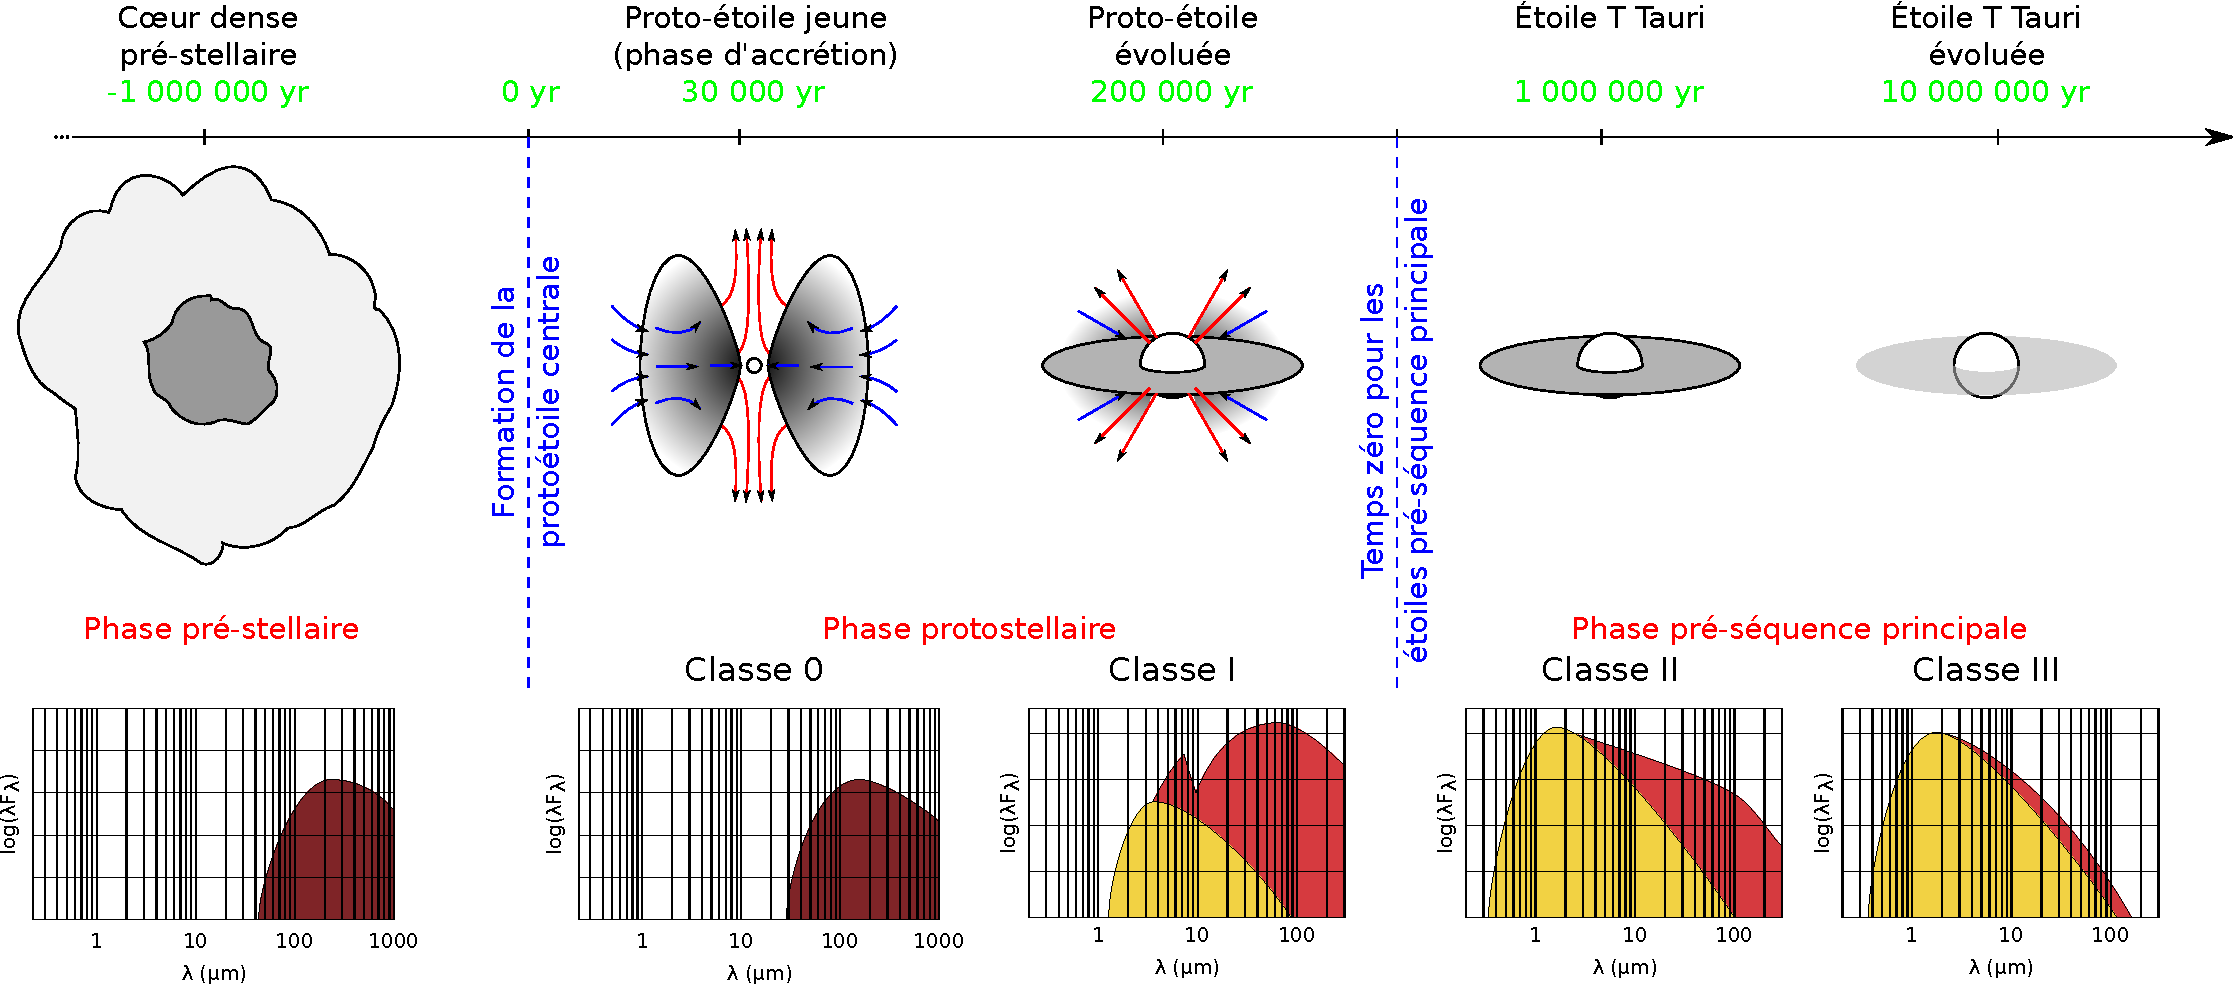
\includegraphics[width=\linewidth]{figure/star_formation.pdf}
\caption[Stades de formation d'une étoile]{Classification empirique des différents stades de formation des étoiles de faible
masse, du cœur dense pré-stellaire à la classe III. Schéma basé sur \citep{andre2002initial}. }\label{fig:star_formation}
\end{figure}


\section{Les disques protoplanétaires}
\subsection{Formation et évolution}
Durant les différentes phases de formation de l'étoile, alors même que le disque de gaz et de poussière se dissipe a lieu la formation des planètes. 

À mesure que le nuage s'effondre sur lui-même, et afin de satisfaire à la conservation du moment cinétique, ce dernier voit sa rotation accélérer, même si la rotation du nuage moléculaire était infime au départ. C'est ainsi que le disque d'accrétion, résultat de l'effondrement du nuage de gaz, est en rotation. L'effondrement d'un nuage moléculaire s'effectuant sur plusieurs ordres de grandeur (en distance), l'accélération de la rotation est d'autant plus grande.

Initialement, il est hautement improbable que le moment cinétique du nuage soit parfaitement nul. C'est ainsi que même si sa rotation est imperceptible lors des premiers stades de son effondrement gravitationnel, le disque d'accrétion fini toujours en rotation. 

\subsection{Évolution hydrodynamique du disque}
\begin{figure}[htbp]
\centering
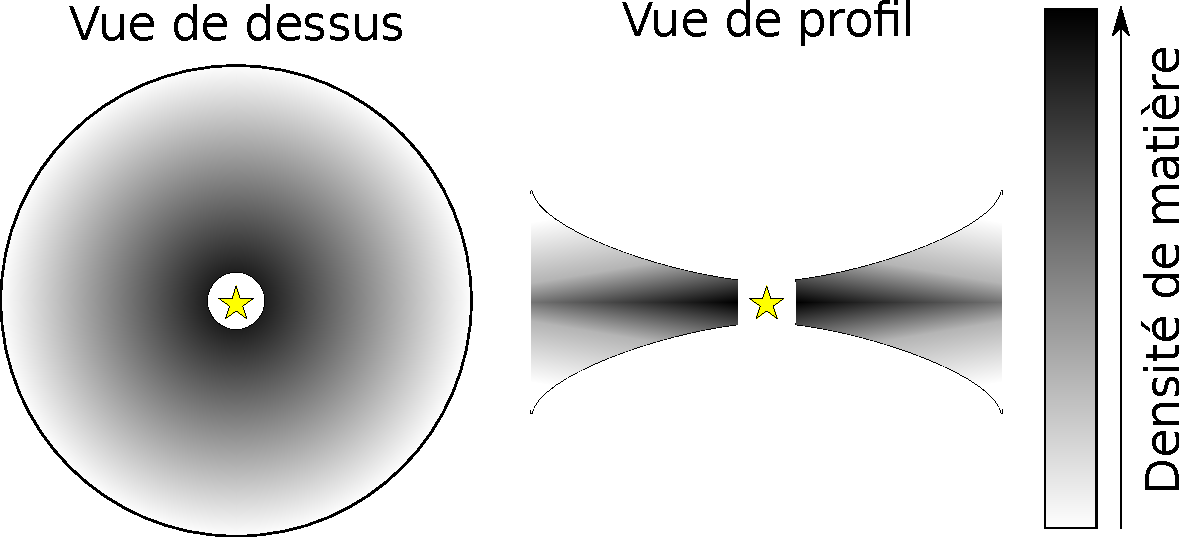
\includegraphics[width=0.6\linewidth]{figure/disk_scheme.pdf}
\caption[Vue de face et de profil d'un disque de gaz.]{Représentation de la répartition radiale et azimutale
de gaz dans un disque protoplanétaire.}\label{fig:disk_scheme}
\end{figure}

Avant de considérer l'évolution d'un disque, il est important de regarder sa masse par rapport à la masse de l'étoile centrale. En effet, si la masse du disque est de l'ordre de la masse de l'étoile, alors des instabilités se développent et on ne peut plus négliger l'autogravité du disque. 

Le \gras{paramètre de Toomre} $Q$, défini par \citep{toomre1964gravitational, goldreich1965gravitational}:
\begin{align}
Q &= \frac{\kappa c_{s}}{\pi G \Sigma}
\end{align}
est un indicateur de la stabilité du disque par rapport à l'auto-gravité. $\kappa$ est la fréquence épicyclique, $c_s$ la vitesse du son, $G$ la constante de gravitation universelle et $\Sigma$ la densité de surface. 

Dans ce paramètre, $\pi G \Sigma$ représente la masse du disque. La vitesse du son $c_{s}$ est liée à la pression thermique ; la \gras[fréquence!epicyclique@épicyclique]{fréquence épicyclique} $\kappa$ détermine quant à elle la force du cisaillement dans le disque.

\bigskip

Si $Q<1$ alors le gaz est instable gravitationnellement et il commence à s'effondrer sur lui-même et à former des sur-densités à
condition que le temps de refroidissement soit inférieur à 3 fois la période orbitale ($\tau_c \lesssim 3 \Omega^{-1}$)
\citep{gammie2001nonlinear}.
Si $Q>1$, le disque est stable.

À partir du paramètre $Q$, on peut dériver une condition sur le rapport de masse entre étoile et disque pour que l'auto-gravité soit négligeable, ce qui donne \citep{gammie2001nonlinear} : 
\begin{align}
\frac{M_\text{d}}{M_\star} &\lesssim \frac{H}{R}
\end{align}
où $M_\text{d}$ et $M_\star$ sont respectivement la masse du disque et de l'étoile. $H=\frac{c_s}{\Omega}$ est l'échelle de hauteur du disque (voir \refsec{sec:disk_properties}) et $R$ la distance par rapport à l'étoile.

Nous ne considérerons que des disques dont la masse $M_\text{d}$ est faible devant la masse de l'étoile $M_\star$. Si tel n'était pas le cas, le temps pour que le disque perde suffisamment de masse pour se retrouver dans le cas qui nous intéresse sera court devant la vie du disque et le temps de formation planétaire. Étant donné qu'on ne s'intéresse qu'aux derniers stades de la formation planétaire, à savoir quand les embryons planétaires ont une masse de l'ordre du dixième de masse terrestre au minimum, il est raisonnable de penser que le disque sera dans un stade peu dense où l'approximation $Q>1$ sera valable.

Dans un tel cas, c'est le potentiel gravitationnel de l'étoile qui domine la dynamique du gaz. En négligeant l'effet de la pression de ce dernier, on peut donc écrire la vitesse angulaire du gaz comme étant égale à la vitesse angulaire képlerienne : 
\begin{align}
\Omega &= \sqrt{\frac{GM_\star}{R^3}}
\end{align}
où $G$ est la constante de gravitation, et $R$ la distance à l'étoile. Dans la pratique, il est à noter que la vitesse est légèrement sous-képlerienne à cause de la pression du gaz. 

\bigskip

Il existe une force de cisaillement entre deux anneaux de gaz concentriques, dûs à leur différence de vitesse. Cette différence de vitesse génère des frottements à cause de la viscosité du disque $\nu$ (dont nous parlerons plus en détail plus loin \refsec{sec:viscosite}) qui chauffe le gaz en lui faisant perdre de l'énergie. Une partie de l'énergie gravitationnelle du gaz est convertie en chaleur, qui est ensuite évacuée par le rayonnement de corps noir du gaz. 

\bigskip

La première conséquence est qu'un terme visqueux va apparaître dans l'équation de l'énergie, comme nous le verrons par la suite. 

La deuxième conséquence, c'est que le gaz perd de l'énergie, et donc dérive lentement vers l'étoile centrale qui accrète petit à petit le gaz du disque. 

On définit donc une vitesse de dérive négative $\vect{v_d} = v_r \hat{e}_r$, orientée vers l'étoile, qui entraine petit à petit le gaz du disque (avec $v_r$ négatif).

Dans la suite, nous allons nous intéresser à la conservation de différentes quantités, que ce soit la masse ou le moment cinétique. Pour cela nous allons définir un anneau de référence, portion du disque sur laquelle nous allons faire le bilan. Le but est ici de présenter d'où viennent les équations et plus précisément d'où viennent les termes des équations. 

\bigskip

Afin de décrire l'évolution hydrodynamique du disque de gaz, nous allons utiliser successivement la \textbf{conservation de la masse}, et la \textbf{conservation du moment cinétique.}. Les démonstrations qui vont suivre ont été déjà faites de nombreuses fois, notamment par \citep{pringle1981accretion}.

\subsubsection{Structure verticale du disque}
On s'intéresse à la répartition de masse verticalement dans le disque. Afin de définir les quantités importantes qui s'y rapportent, nous allons écrire l'équation de l'équilibre hydrostatique. On a alors :
\begin{align}
\inv{\rho}\dpd{P}{z} &= \vect{g}.\hat{e}_z\\
&= \left(-\frac{GM}{R^3}\hat{e}_r\right).\hat{e}_z
\end{align}

$\vect{g}$ est orienté vers l'étoile centrale, selon la direction $r$ (en sphérique). En projetant sur l'axe $z$ pour effectuer le produit scalaire, et en faisant l'approximation que $r\sim a$ on obtient alors :
\begin{align}
\inv{\rho}\dpd{P}{z} &= -\Omega^2 z
\end{align}

En considérant un disque isotherme selon $z$ et d'après la loi des gaz parfaits
\begin{align}
P &= \frac{\rho k_B T}{\mu m_H}
\end{align}
il vient
\begin{align}
\dpd{\rho}{z} &= -\frac{\mu m_H\Omega^2}{k_B T}\rho z
\end{align}

On obtient alors :
\begin{align}
\rho(z) &= \rho_0\exp\left(-\frac{z^2}{2H^2}\right)
\end{align}
où $\rho_0$ est la densité volumique du disque de gaz dans le plan médian et $H$ l'échelle de hauteur du disque est définie par (dans la limite isotherme) : 
\begin{align}
H &= \sqrt{\frac{k_B T}{\Omega^2 \mu m_H}}
\end{align}

\bigskip

Sachant que la vitesse du son est définie par :
\begin{align}
{c_s}^2=\frac{P}{\rho} &= \frac{k_B T}{\mu m_H}
\end{align}
dans le cas d'un gaz parfait, on peut alors écrire la relation suivante entre l'échelle de hauteur et la vitesse du son : 
\begin{align}
c_s &= H\Omega
\end{align}

\bigskip

On considèrera dans la suite les quantités moyennées selon $z$, et en particulier on définit la densité de surface $\Sigma$ de
la façon suivante : 
\begin{align}
\Sigma &= \int_{-\infty}^{+\infty} \rho \dif z\nonumber\\
&=\rho_0 \int_{-\infty}^{+\infty}  \exp\left(-\frac{z^2}{2H^2}\right)\dif z\nonumber\\
\Sigma &= \sqrt{2\pi}\rho_0 H\label{eq:surface-to-volume}
\end{align}

% fromang & nelson 2006 donnent une formule, après l'équation (20), mais elle ne correspond pas à ça, peut-être lié à un truc magnétique ou je sais pas quoi

\subsubsection{Bilan de masse}
\begin{figure}[htbp]
\centering
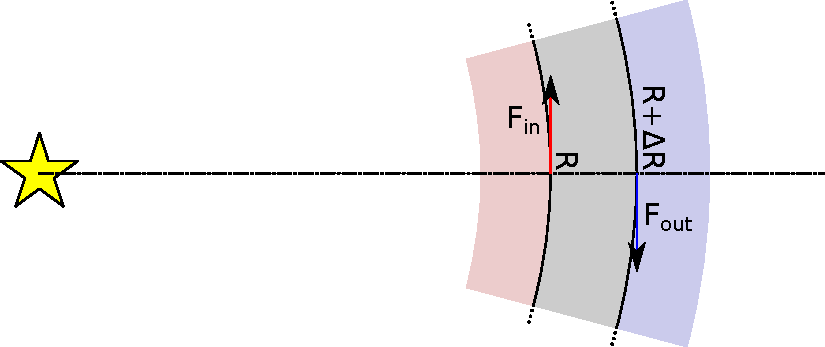
\includegraphics[width=0.7\linewidth]{figure/disk_ring.pdf}
\caption[Bilan de moment cinétique d'un anneau d'épaisseur $\Delta R$.]{Représentation d'un anneau de largeur $\Delta R$ et du
bilan de moment cinétique de ce dernier.}\label{fig:disk_ring}
\end{figure}

On cherche dans un premier temps à faire le bilan de masse de l'anneau considéré. Sa masse s'écrit :
\begin{align}
m_a &= 2\pi R \Delta R \Sigma(R)\label{eq:m_a}
\end{align}

\bigskip

Soit $v_r\hat{e}_r$ la vitesse radiale du gaz (avec $v_r<0$ dans notre cas). Cette vitesse est responsable d'un certain taux d'accrétion du gaz du disque sur l'étoile centrale. On cherche maintenant à modéliser cette accrétion pour le bilan de moment cinétique sur l'anneau.

Pour cela, on cherche à exprimer la variation de masse de l'anneau, ainsi que le moment cinétique emporté par cette variation de masse. 

Au bord interne $R$, par unité de temps, la masse entrant ou sortant de l'anneau peut-être exprimée comme un flux :
\begin{align}
\dif F_M &= \Sigma \cdot 2\pi R \cdot \left( -\vect{v_r} \cdot \vect{\dif S} \right)
\end{align}
En effet, en multipliant la circonférence de l'anneau par la vitesse, on obtient une sorte de surface par unité de temps qui représente ce qui sort de la frontière virtuelle représentée par l'anneau en $r=R$. 

Le flux de matière doit être négatif si la masse sort de l'anneau. Les éléments de surface étant orientés vers l'extérieur, un vecteur vitesse colinéaire à $\vect{\dif S}$ implique que la matière sort de l'anneau. Ceci explique la présence du signe négatif dans l'expression du flux de matière.

On a ainsi aux deux bords de l'anneau :
\begin{subequations}
\begin{align}
\dif F_M(R) &= \Sigma(R) \cdot 2\pi R \cdot v_r(R)\\
\dif F_M(R+\Delta R) &= - 2\pi (R+\Delta R) \cdot v_r(R+\Delta R) \cdot \Sigma(R+\Delta R)
\end{align}\label{eq:dif_F_M}
\end{subequations}
$v_r$ étant négatif, on a bien une perte de masse en $r=R$ et un gain de masse en $r=R+\Delta R$.

La conservation de la masse implique alors que la dérivée temporelle de la masse de l'anneau est égale au flux de masse à travers sa surface. On a ainsi : 
\begin{align*}
\dpd{}{t}\left(2\pi R \Delta R \Sigma(R)\right) &= \dif F_M(R) + \dif F_M(R+\Delta R)
\end{align*}

En faisant tendre l'épaisseur $\Delta R$ de l'anneau vers 0, on obtient alors :
\begin{important}
\begin{align}
\dpd{\Sigma}{t} + \inv{R}\dpd{}{R}\left(R v_r \Sigma\right)&=0\label{eq:conservation_masse}
\end{align}
\end{important}

\subsubsection{Bilan de moment cinétique/angulaire}
On fait maintenant un bilan des variations de moment cinétique pour l'anneau de gaz. Pour cela on dit que la variation de moment
cinétique (que l'on écrit en dérivant $J_a(t)$) est égale aux variations de moment cinétique induites aux bords de l'anneau par
échange de masse à laquelle s'ajoute la différence entre les deux couples visqueux qui s'appliquent au bord externe et interne.
Ce qui donne : 
\begin{align}
\dod{J_a}{t} &= \dif J(R+\Delta R) + \dif J(R) + \Gamma_\text{out} - \Gamma_\text{in}\label{eq:cons_J_a}
\end{align}

Le moment cinétique de l'anneau est défini par :
\begin{align}
\vect{J_a} &= \vect{R} \wedge (m_a\vect{v(R)}) \nonumber\\
\vect{J_a} &= 2\pi R^3 \Delta R \Sigma(R)\Omega(R)\hat{e}_z\label{eq:J_a}
\end{align}
où $\Sigma$ et $\Omega$ sont la densité de surface et la vitesse angulaire du gaz à la position $R$ dans le disque.

Le flux de moment cinétique est simplement défini comme la quantité de moment cinétique emportée ou apportée par le flux de masse défini précédemment \refeq{eq:dif_F_M} :
\begin{subequations}
\begin{align}
\dif J(R) &= 2\pi v_r(R) \Sigma(R)\cdot R^3\Omega(R)\hat{e}_z\label{eq:dJ_in}\\
\dif J(R+\Delta R) &= -2\pi v_r(R+\Delta R) \Sigma(R+\Delta R)\cdot \left(R+\Delta R\right)^3\Omega(R+\Delta R)\hat{e}_z\label{eq:dJ_out}
\end{align}\label{eq:dJ}
\end{subequations}

\bigskip

À ceci s'ajoute la variation de moment cinétique induite par la friction entre anneaux concentriques, en d'autres termes, dus à la viscosité du disque. Cette variation de moment cinétique est représentée sous la forme d'un couple exercé par les anneaux internes et externes à celui considéré. 

La force visqueuse par unité de longueur est définie par :
\begin{align}
\dif F_\text{vis} &= \nu \Sigma A = \nu \Sigma R \dod{\Omega}{R}
\end{align}
où $A=R \dod{\Omega}{R}$ est le taux de cisaillement.

La force visqueuse induite par les anneaux entourant l'anneau considéré est alors : 
\begin{subequations}
\begin{align}
\vect{F_\text{in}}(R)&= 2\pi\nu \Sigma R^2 \dod{\Omega}{r}(R) \hat{e}_\theta\\
\vect{F_\text{out}}(R+\Delta R)&= 2\pi\nu \Sigma (R+\Delta R)^2 \dod{\Omega}{r}(R+\Delta R) \cdot (-\hat{e}_\theta)
\end{align}
\end{subequations}
L'anneau interne tournant plus vite, la force est dirigée dans le sens de rotation $\hat{e}_\theta$. À l'inverse, l'anneau externe tourne moins vite, il tend à freiner l'anneau de référence et s'oppose à son mouvement. La force est donc opposée au sens de rotation.

\bigskip

Ainsi, le couple $\vect{\Gamma}=\vect{R}\wedge\vect{F}$ issu de chacun des anneaux entourant celui de référence s'écrit :
\begin{subequations}
\begin{align}
\vect{\Gamma_\text{in}} &= 2\pi\nu \Sigma R^3 \dod{\Omega}{R}(R) \hat{e}_z\label{eq:G_in}\\
\vect{\Gamma_\text{out}} &= -2\pi\nu \Sigma (R+\Delta R)^3 \dod{\Omega}{R}(R+\Delta R) \hat{e}_z\label{eq:G_out}
\end{align}\label{eq:J_torques}
\end{subequations}

\bigskip

En utilisant \refeq{eq:J_a}, \refeq{eq:dJ}, \refeq{eq:J_torques}, dans \refeq{eq:cons_J_a} il vient alors :
\begin{align}
\dpd{\Sigma}{t} &= \inv{R}\dpd{}{R}\left\{\inv{\dpd{}{R}\left(R^2\Omega\right)} \dpd{}{R}\left[\nu \Sigma R^3 \left(-\dod{\Omega}{R}\right)\right]\right\}
\end{align}

Dans le cas d'un disque képlerien ($\Omega = \sqrt{\frac{GM}{R^3}}$) on obtient finalement :
\begin{important}
\begin{align}
\dpd{\Sigma}{t} &=\frac{3}{R}\dpd{}{R}\left[\sqrt{R} \dpd{}{R}\left(\nu \Sigma R^\sfrac{1}{2}\right)\right]\label{eq:diffusion_equation}
\end{align}
\end{important}

Le calcul détaillé est disponible \refsec{app:equation_angular_momentum}.

Cette équation a nécessité les approximations suivantes : 
\begin{enumerate}
\item On suppose que le potentiel gravitationnel est indépendant du temps ($\dod{\Omega}{t}=0$), c'est-à-dire que la masse de l'étoile est constante, l'accrétion ayant un effet négligeable.
\item On suppose que le mouvement du gaz est képlerien $\Omega=\sqrt{\frac{GM}{r^3}}$, ce qui n'est pas rigoureusement vrai, la pression du gaz rendant le mouvement légèrement sous-képlerien.
\end{enumerate}

\subsubsection{Temps de vie et dispersion du disque}\label{sec:dispersion}\index{dissipation du disque}

\begin{figure}[htbp]
\centering
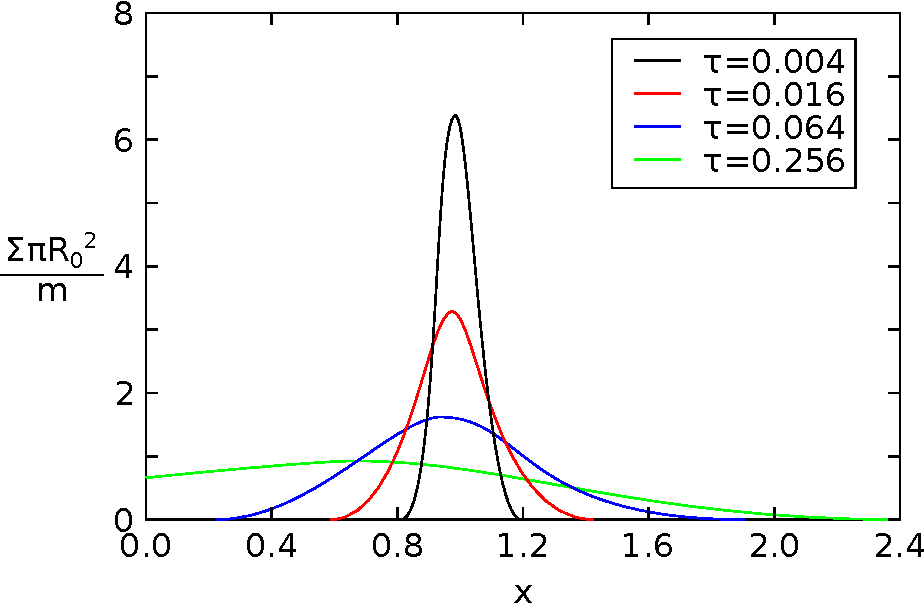
\includegraphics[width=0.65\linewidth]{figure/pringle_viscous_dissipation.pdf}
\caption[Évolution visqueuse d'un anneau de matière]{Évolution visqueuse d'un anneau de matière de masse $m$ et de rayon $R_0$.
La densité de surface est montrée comme une fonction de la longueur dédimensionnée $x=R/R_0$ et du temps adimensionné
$\tau=12\nu t / {R_0}^2$.}\label{fig:pringle_viscous_dissipation}
\end{figure}

Cette équation permet de modéliser l'évolution visqueuse d'un disque au cours du temps. \reffig{fig:pringle_viscous_dissipation}, tirée de \cite{pringle1981accretion} et recalculée illustre l'évolution visqueuse d'un anneau de matière de masse $m$ dans des unités adimensionnées de distance et de temps.

\bigskip

On situe généralement le temps de vie d'un disque protoplanétaire autour de quelques millions d'années. Cette information est
obtenue de plusieurs études d'amas d'étoiles d'âges différents dans lesquelles on mesure le taux d'étoiles possédant un excès
infrarouge (signe de présence d'un disque) \citep{williams2011protoplanetary}. 70\% à 80\% des étoiles jeunes ($t<1\unit{Myr}$)
possèdent un disque \citep{winston2007combined, gutermuth2008spitzer}, 40 à 50\% des étoiles dans des amas d'âge compris entre 2
et 3 millions d'années en possèdent un \citep{lada2006spitzer, sung2009spitzer} tandis que moins de 20\% des étoiles dans des
amas d'environ 5 millions d'années ont un disque \citep{currie2009last}. 

Par la rareté des disques en train de se dissiper, les observations suggèrent aussi que les disques se dissipent très rapidement, avec un temps de dispersion d'environ $10^5$ ans \citep{simon1995disk, wolk1996search}. La dissipation visqueuse n'explique alors pas comment le disque peut subsister pendant plusieurs millions d'années, mais se dissiper complètement en \nombre{500 000} ans. \cite{clarke2001dispersal} ont montré qu'il était possible d'expliquer ce comportement à deux temps caractéristiques à l'aide de la photo-évaporation. 

\begin{figure}[htbp]
\centering
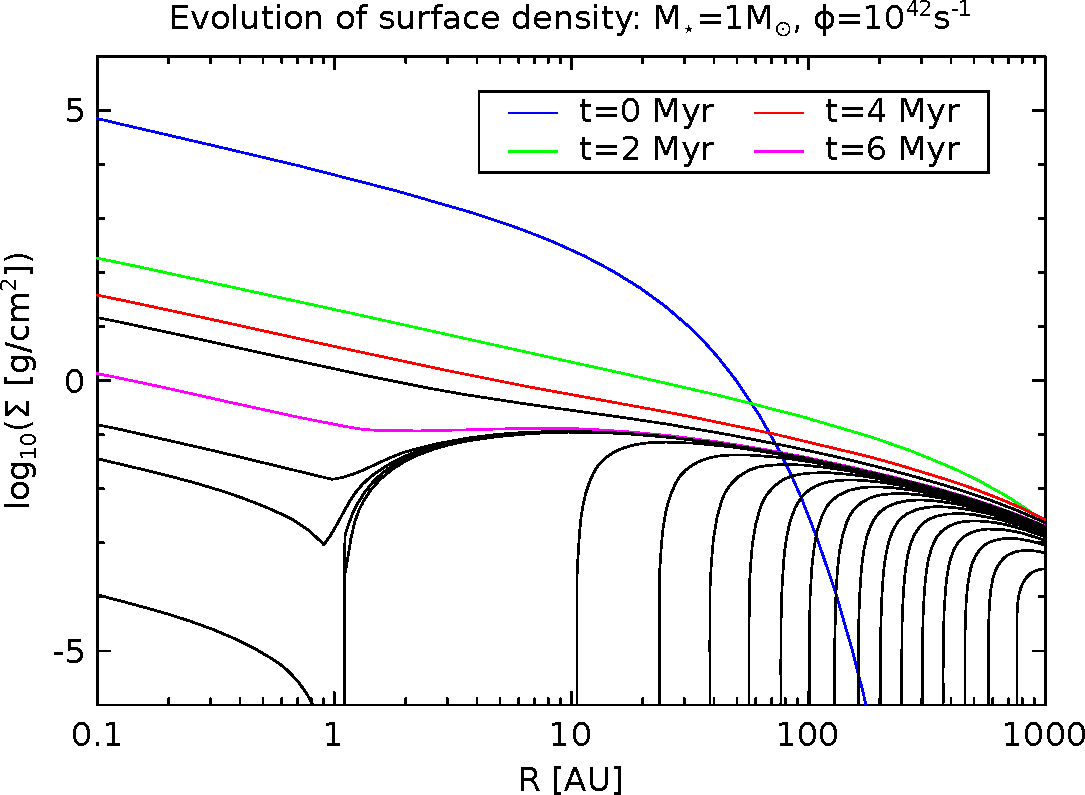
\includegraphics[width=0.65\linewidth]{figure/disk_dispersion.pdf}
\caption[Dissipation du disque]{Évolution de la densité de surface en fonction du temps dans une simulation qui modélise la
dissipation du disque protoplanétaire par évolution visqueuse et photo-évaporation. À $t=6.20\unit{Myr}$ le disque est
totalement dissipé. Figure adaptée de \cite{alexander2006photoevaporation}.}\label{fig:disk_dispersion}
\end{figure}

Le principe de la \gras{photo-évaporation} est que le rayonnement de l'étoile permet de dissocier le dihydrogène ainsi que de fournir de l'énergie cinétique aux atomes du gaz. À partir d'un rayon dit \og rayon gravitationnel\fg $r_g$ qui représente la distance à partir de laquelle l'énergie fournie par les photons de l'étoile devient suffisante pour contrebalancer les effets de sa gravité, la photo-évaporation permet d'évaporer une partie du gaz superficiel du disque. Le disque va alors se creuser jusqu'à séparer le disque en deux. Les parties internes du disques ne sont alors plus alimentées par les parties externes. Des simulations montrent que les parties externes se dispersent rapidement une fois les parties internes accrétées \citep{alexander2006photoevaporation}. \reffig{fig:disk_dispersion} montre l'évolution du profil radial de densité en fonction du temps en présence de l'évolution visqueuse et de la photo-évaporation.

La photo-évaporation est aussi possible par l'irradiation d'étoiles massives (étoiles OB) dans le voisinage du disque \citep{adams2004photoevaporation}.

\subsection{Profil de température}
Du point de vue de la température, il y a principalement deux types de disques : 
\begin{itemize}
\item les \gras[chauffage visqueux]{disques actifs} : la source de température est le disque lui-même, qui par \gras{chauffage visqueux} (frottements) va convertir de l'énergie gravitationnelle en chaleur ;
\item les \gras[irradiation]{disques passifs} : la source de chaleur/température est l'étoile centrale qui éclaire le disque. 
\end{itemize}

Un disque peut à la fois être actif et passif, mais généralement on essaie d'approximer, de considérer que l'un est négligeable devant l'autre. De plus, un disque aura des zones actives et des zones passives, c'est-à-dire que certaines zones seront principalement chauffées par la viscosité alors que d'autres le seront par l'\gras[irradiation]{irradiation de l'étoile}.

\bigskip

Afin de déterminer le profil de température, il faut écrire l'équation de conservation de l'énergie, qui va tenir compte de tous les termes source et toutes les pertes, par unité de surface.

On a tout d'abord les pertes par rayonnement de corps noir. Ensuite, il y a les termes sources. Pour un disque actif, le terme source est le chauffage visqueux. Pour un disque passif, c'est l'irradiation de l'étoile \citep{chiang1997spectral}. Dans notre cas, il y a un terme dû à l'enveloppe du disque, un dû à l'irradiation de l'étoile centrale, et enfin un dernier dû au chauffage visqueux.


\begin{figure}[htbp]
\centering
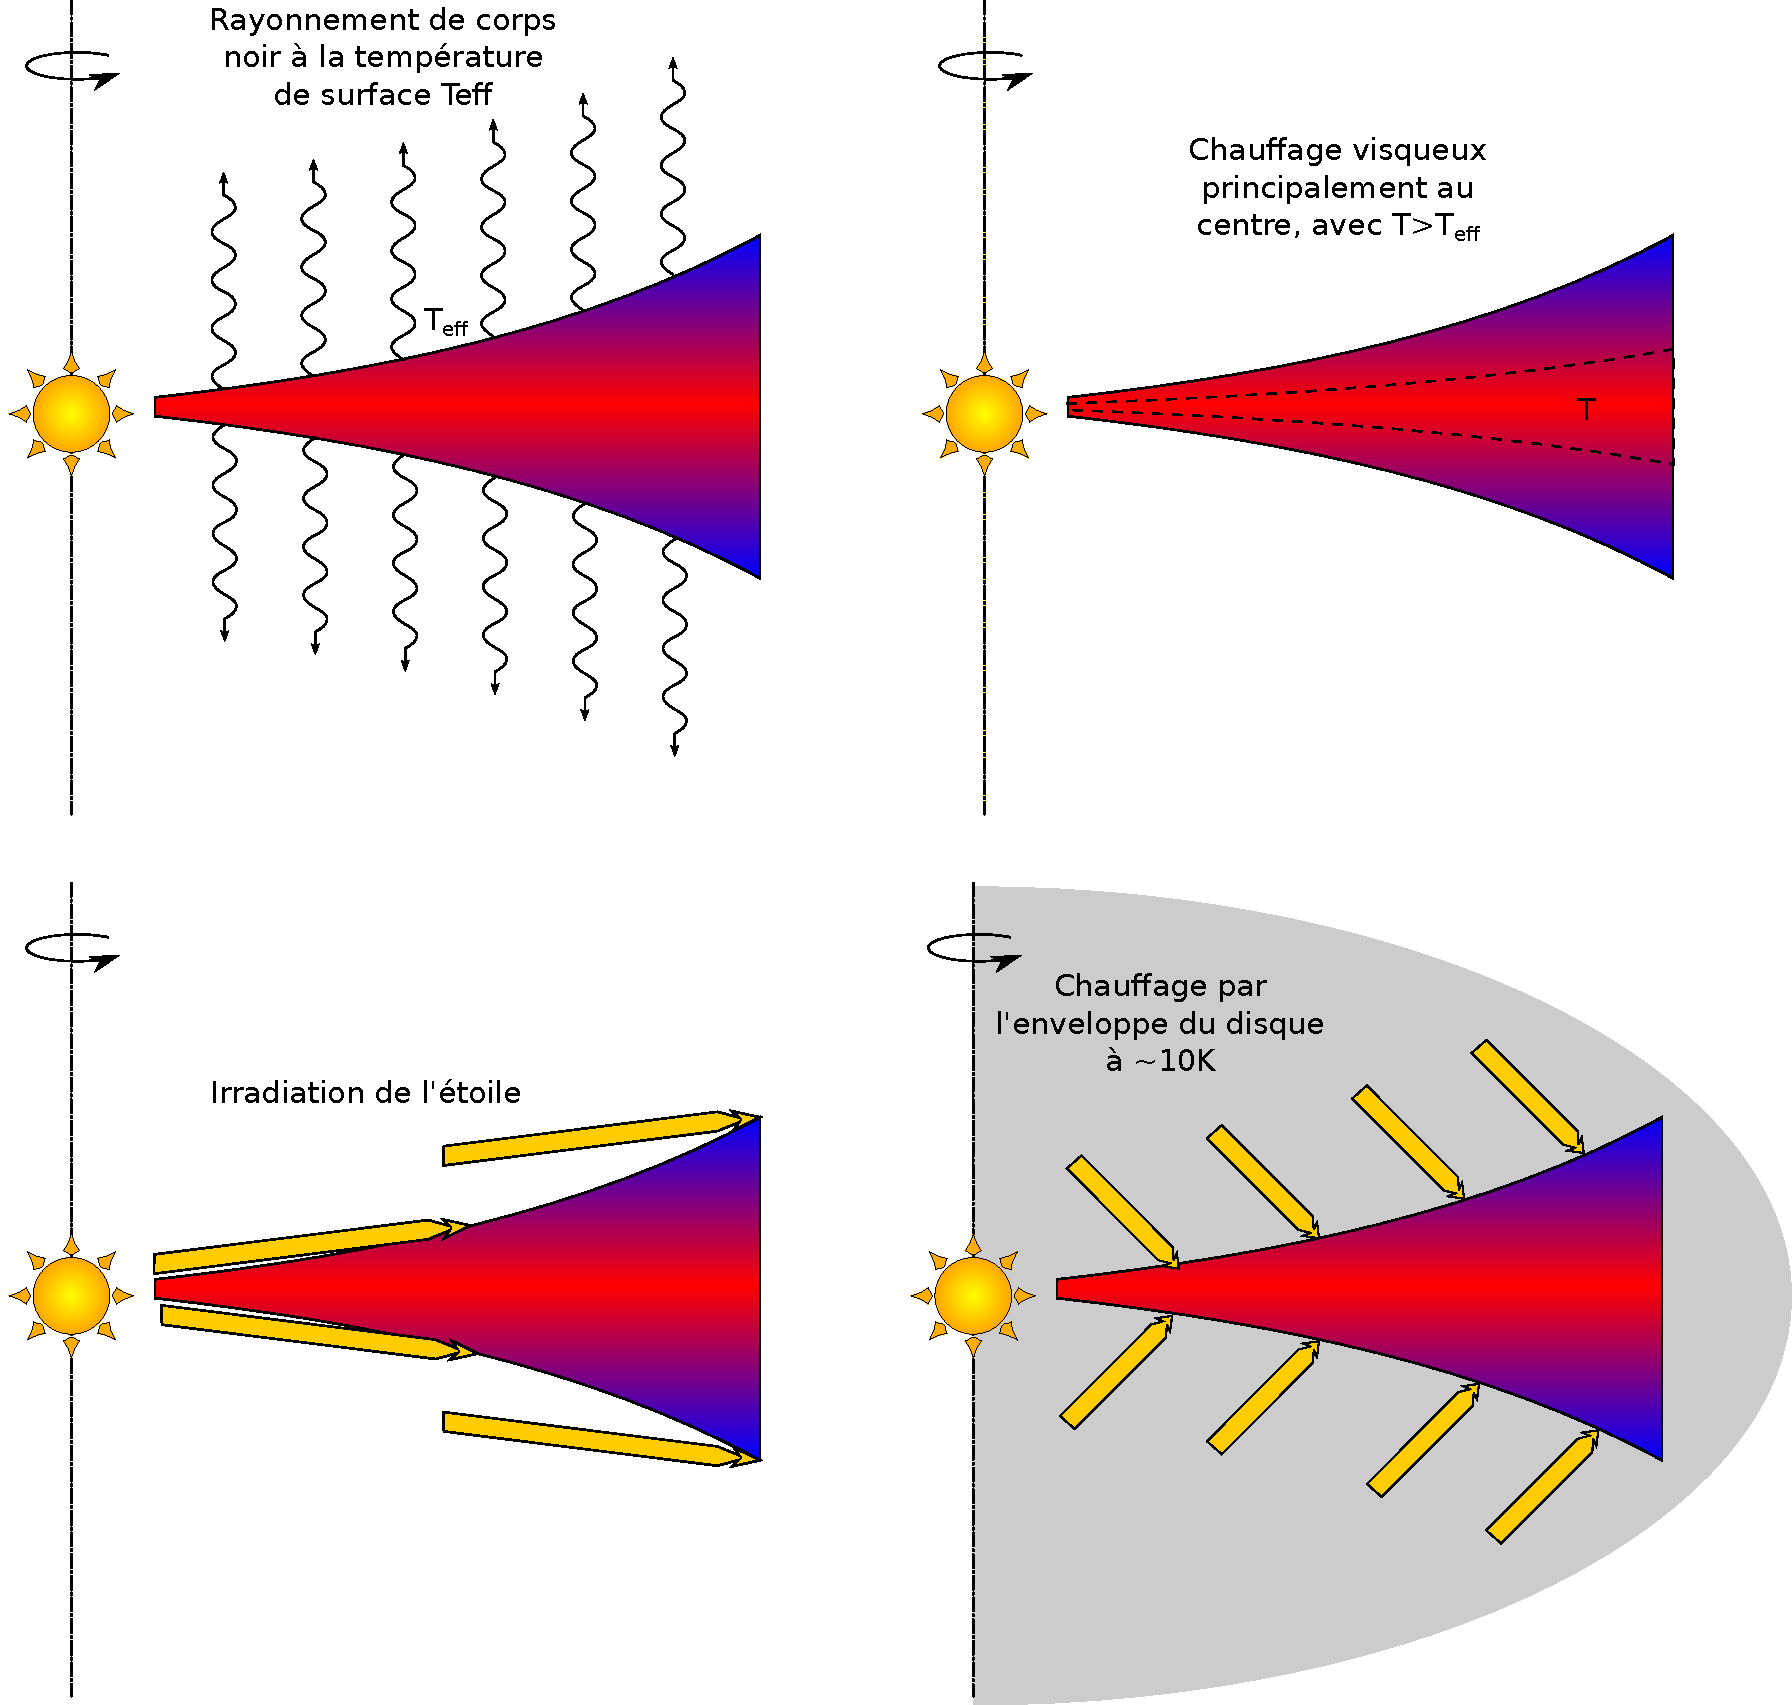
\includegraphics[width=0.65\linewidth]{figure/disk_energy.pdf}
\caption[Bilan énergétique d'un disque.]{Représentation du bilan thermique d'un disque}\label{fig:energy_equilibrium}
\end{figure}

\subsubsection{Refroidissement radiatif}
Par toute la surface du disque, qui est à une température $T_\text{eff}$ en surface, on a des pertes par rayonnement de corps noir : 
\begin{align}
P_\text{cn} &= - 2\sigma {T_\text{eff}}^4
\end{align}
où $\sigma$ est la constante de Stefan-Boltzmann. Ces dernières doivent être multipliées par deux, en effet, il y a des pertes
par rayonnements des deux cotés du disque à une position donnée. 

\bigskip

$T_\text{eff}$ est une estimation de la température effective du disque à sa surface \cite{hubeny1990vertical} : 
\begin{subequations}
\begin{align}
{T_\text{eff}}^4 &= \frac{T^4}{\tau_\text{eff}}
\intertext{avec}
\tau_\text{eff} &= \frac{3}{8}\tau + \frac{\sqrt{3}}{4} + \inv{4\tau}
\end{align}
\end{subequations}
où $\tau=\kappa\Sigma/2$ est la profondeur optique verticale moyenne, $\kappa$ étant l'opacité du disque (l'opacité sera détaillée dans \refsec{sec:opacity}).

Cette température effective est le résultat d'un transfert de rayonnement depuis le cœur du disque, à une température $T$ qui se refroidit, et chauffe les différentes couches successives jusqu'à atteindre le bord du disque. Il résulte alors une température $T_\text{eff}$ plus faible que la température dans le plan du disque. 

\subsubsection{Chauffage par l'enveloppe}
\begin{figure}[htbp]
\centering
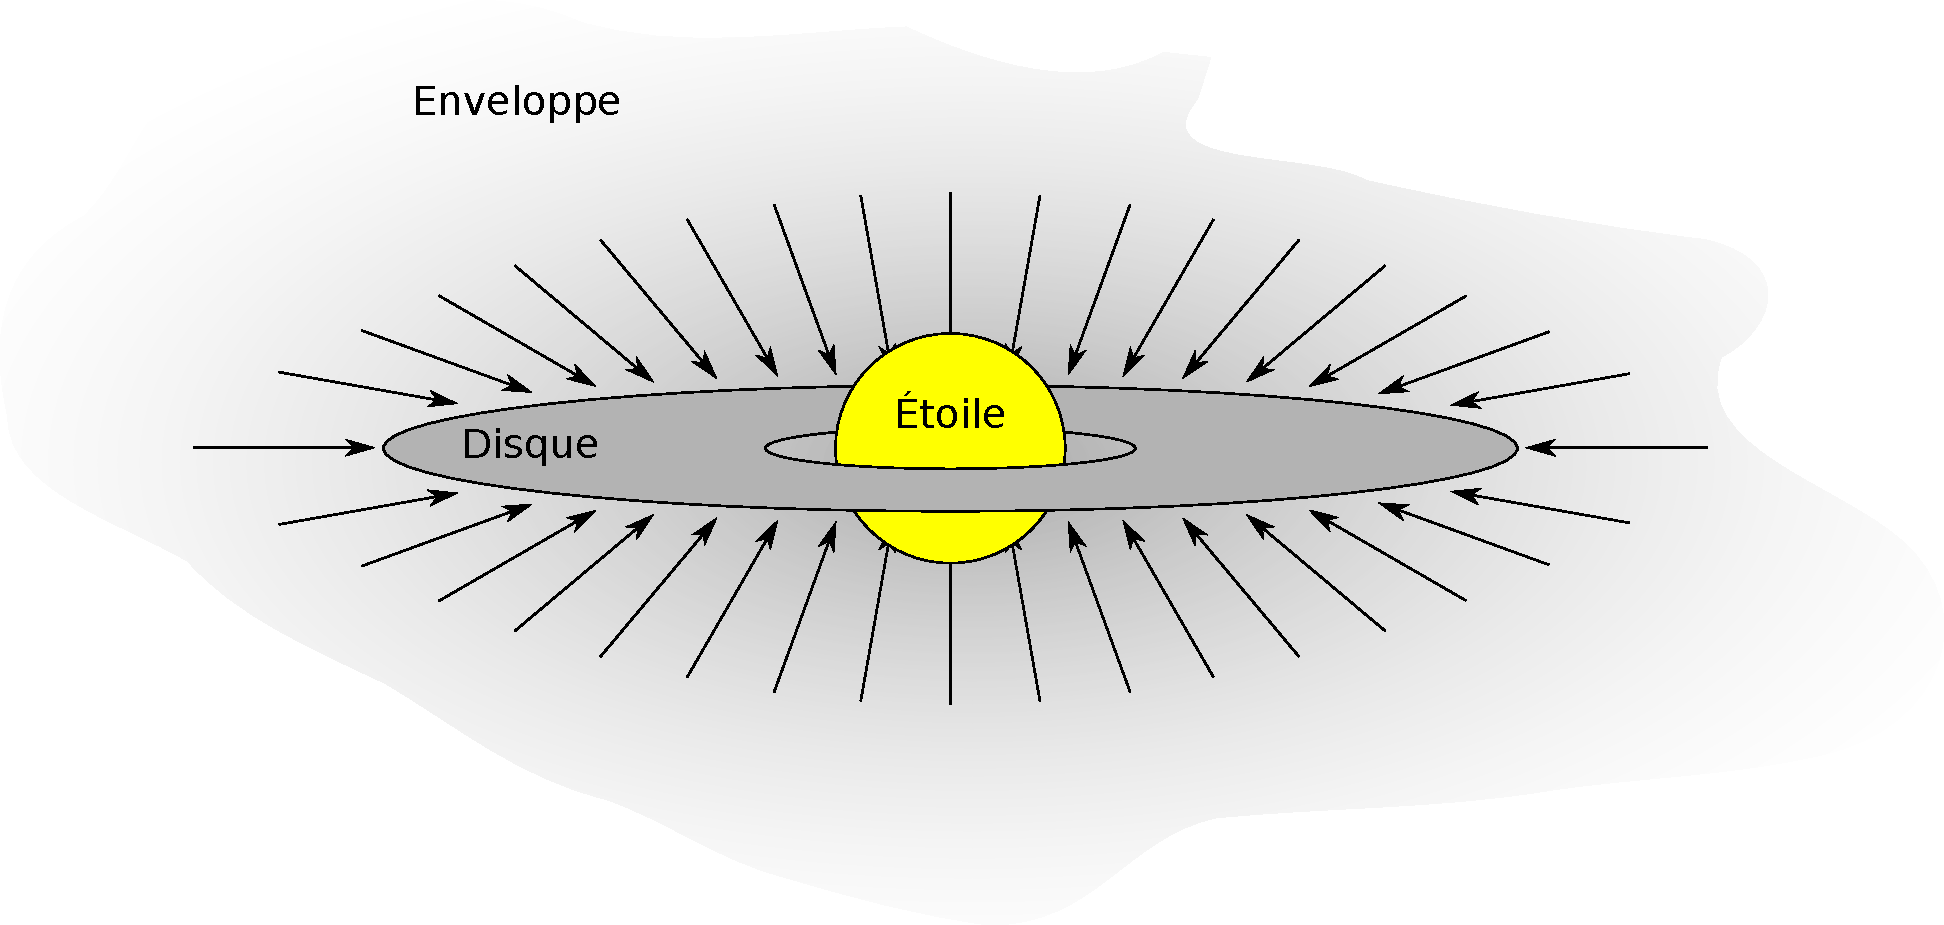
\includegraphics[width=0.65\linewidth]{figure/disk_envelope.pdf}
\caption[Chauffage du disque par l'enveloppe]{Représentation de l'effondrement d'un nuage moléculaire et des différentes parties
qui composent le système en effondrement.}\label{fig:envelope}
\end{figure}
L'enveloppe \reffig{fig:envelope} provient de l'effondrement continu du nuage moléculaire. C'est un reste diffus qui alimente continuellement le disque en matière. Mais cette enveloppe, qui possède une température que l'on fixe ici à $T_\text{en} = 10\unit{K}$ contribue aussi au bilan d'énergie du disque en apportant la contribution uniforme suivante :
\begin{align}
C_\text{en} &= 2 \sigma {T_\text{en}}^4
\end{align}

La température de l'enveloppe étant très faible, cette dernière ne contribue que dans les parties externes du disque, là où la densité de surface du gaz est très faible, rendant du même coup le chauffage visqueux extrêmement ténu lui aussi.

\subsubsection{Chauffage par l'étoile}\label{sec:irradiation}\index{irradiation}
La surface du disque reçoit de la lumière de l'étoile centrale. Soit $R_\star$, $L_\star$ respectivement le rayon et la
luminosité de l'étoile. Soit $\varepsilon$ l'albédo du disque, que l'on choisit typiquement égal à $0.5$  \citep{menou2004low}. 

Le flux incident est alors \citep[eq. (7)]{menou2004low} : 
\begin{align}
F_\text{irr} &= \frac{L_\star(1-\varepsilon)}{4\pi r^2} \alpha
\end{align}
où $\alpha$ (avec $\alpha\ll 1$) représente l'angle entre les rayons incidents et la surface du disque. 

D'après notamment \cite[eq. (5)]{chiang1997spectral}, cet angle peut être écrit comme : 
\begin{align}
\alpha &= 0.4 \frac{R_\star}{r} + r \dod{}{r}\left(\frac{H}{r}\right)
\end{align}

On note que dans cette expression, le premier terme illustre le fait que l'étoile n'est pas ponctuelle, et que ceci a un effet sur l'irradiation dès que l'on s'approche de cette dernière. Le deuxième terme représente la surface du disque qui intercepte le rayonnement incident, et qui est fonction de la variation d'échelle de hauteur du disque (plus le disque est évasé, et plus la paroi qui intercepte le rayonnement est abrupte). 

Il vient enfin, en exprimant la luminosité de l'étoile en fonction de sa température et de son rayon, l'expression suivante :
\begin{align}
C_\text{irr} &= 2 \sigma {T_\star}^4 \frac{{R_\star}^2}{r^2} (1-\varepsilon) * \left[0.4 \frac{R_\star}{r} + r \dod{}{r}\left(\frac{H}{r}\right)\right]
\end{align}

Il faut cependant noter qu'une approximation implicite a été faite en supposant que $h_p\sim h$, où $h_p$ est la position
verticale dans le disque où les photons stellaires sont absorbés. En effet, l'absorption des photons ne dépend pas uniquement de
la densité, mais aussi de l'opacité du disque aux photons stellaires, qui elle-même varie suivant la composition
composition du disque.

Dans le cadre d'un disque optiquement épais, il devient possible de considérer $h_p \sim h$.

%non ponctualité de l'étoile : Chiang & Goldreich, 1997, ApJ, 490, 368
%expression de l'angle notammenet : dullemond 2000
%autres expressions : menou & goodman 2004

\subsubsection{Chauffage visqueux}\index{chauffage visqueux}
On considère un fluide incompressible. Il peut paraître étonnant de considérer un disque de gaz comme étant un fluide incompressible. Mais en fait l'aspect compressible va surtout se manifester lors de la mise à l'équilibre, générant des ondes de chocs par exemple. Mais une fois le disque stabilisé tout se passe comme si on avait un fluide incompressible. C'est matérialisé par le fait que la vitesse dans le disque est considérée comme inférieure à la vitesse du son dans le milieu $c_s$, au delà de laquelle on aura des ondes des choc ayant une incidence sur le bilan thermique. Ainsi donc, en considérant un fluide incompressible, on peut partir de l'expression de la variation d'énergie cinétique (qui est l'inverse du chauffage, les pertes cinétiques étant converties en chaleur par la viscosité) \citep[(16.3)]{landau1989mecanique} : 
\begin{align}
\dpd{E_c}{t} &= - \frac{1}{2}\int \eta(T_{ik})^2\dif V\\
T_{ik} &= \left(\dpd{v_i}{x_k} + \dpd{v_k}{x_i}\right)\nonumber
\end{align}
où $\eta = \rho\nu$ est la viscosité dynamique\footnote{$\nu$ étant la viscosité cinématique et $\rho$ la densité volumique de gaz.}

À partir de \citep[(15.8) et (15.17)]{landau1989mecanique}, on extrait de manière assez directe l'expression du tenseur $T_{ik}$ en coordonnées cylindriques : 
\begin{align}
T_{rr} &= 2\dpd{v_r}{r}, & T_{r\varphi} &= \left(\inv{r} \dpd{v_r}{\varphi} + \dpd{v_\varphi}{r} - \frac{v_\varphi}{r}\right),\nonumber\\
T_{\varphi\varphi} &= 2 \left(\inv{r} \dpd{v_\varphi}{\varphi} + \frac{v_r}{r}\right), & T_{\varphi z} &= \left(\dpd{v_\varphi}{z} + \inv{r}\dpd{v_z}{\varphi}\right),\\
T_{zz} &= 2\dpd{v_z}{z}, & T_{rz} &= \left(\dpd{v_z}{r} + \dpd{v_r}{z}\right).\nonumber
\end{align}
sachant que le tenseur est symétrique en statique, ce qui donne : 
\begin{align}
T_{ik} &= \begin{pmatrix}
T_{rr} & T_{r\varphi} & T_{rz}\\
T_{r\varphi} & T_{rr} & T_{\varphi z}\\
T_{rz} & T_{\varphi z} & T_{zz}
\end{pmatrix}
\end{align}

À partir de ces expressions, nous allons procéder à quelques simplifications, moyennant quelques approximations : 
\begin{itemize}
\item On considère tout d'abord que $v_z=0$ en invoquant le fait que le disque est à l'équilibre hydrostatique verticalement. 

\item Ensuite, on néglige tous les termes en $\pd{}{\varphi}$ car le disque est axisymétrique. 

\item On néglige enfin tous les termes en $v_r$ devant les termes en $v_\varphi$ étant donné que la vitesse de dérive (liée à l'accrétion) est beaucoup plus petite que la vitesse de rotation due au mouvement képlerien. En effet, la vitesse de dérive est une conséquence des pertes d'énergie par frottement visqueux entre deux anneaux due à la différence de vitesse de leur mouvement képlerien.
\end{itemize}

Seul le terme $T_{r\varphi}$ reste :
\begin{align}
T_{r\varphi} &= \dpd{v_\varphi}{r} - \frac{v_\varphi}{r}\nonumber\\
\intertext{avec $v_\varphi=r\Omega$}
T_{r\varphi} &= r\dod{\Omega}{r}
\end{align}

Il vient alors :
\begin{align*}
\dpd{E_c}{t} &= - \frac{1}{2}\int \eta(T_{ik})^2\dif V\\
&= - \frac{1}{2}\int \eta\sum_{i=1}^3\sum_{j=1}^3 {T_{ij}}^2\dif V\\
&= - \frac{1}{2}\int \eta\left({T_{r\varphi}}^2+{T_{\varphi r}}^2\right)\dif V\\
\intertext{Le tenseur est symétrique, on a donc $T_{r\varphi} = T_{\varphi r}$}
&= - \frac{1}{2}\int \eta\left(2{T_{r\varphi}}^2\right)\dif V\\
&= - \iint \rho\nu \left(r\dod{\Omega}{r}\right)^2\dif S\dif z\\
\intertext{En utilisant une vitesse angulaire képlerienne $\Omega=\sqrt{\frac{GM}{r^3}}$ on obtient alors :}
&= - \int \Sigma\nu \left(-\frac{3}{2}\Omega\right)^2\dif S\\
\dpd{E_c}{t} &= - \frac{9}{4} \int \Sigma\nu \Omega^2\dif S
\end{align*}

La variation d'énergie cinétique est négative, cette perte est convertie en chaleur par chauffage visqueux. Le chauffage visqueux intégré sur toute la surface du disque peut ainsi être défini comme : 
\begin{align*}
C_\text{vis/tot} &= - \dpd{E_c}{t}
\end{align*}
de sorte qu'on peut écrire le chauffage visqueux par unité de surface comme étant égal à :
\begin{align}
C_\text{vis} &= \frac{9}{4} \nu\Sigma\Omega^2
\end{align}

\subsubsection{Bilan}
On cherche maintenant la température d'équilibre du disque, compte tenu de tous les termes rentrant dans l'équation bilan de l'énergie du disque. Il vient alors, en considérant le chauffage visqueux, l'irradiation de l'étoile centrale, le chauffage par l'enveloppe et les pertes par radiation à la surface du disque : 
\begin{align}
0 &= P_\text{cn} + C_\text{en} + C_\text{irr} + C_\text{vis}\nonumber\\
0 &= - 2\sigma \frac{T^4}{\frac{3}{8}\tau + \frac{\sqrt{3}}{4} + \inv{4\tau}} + 2 \sigma {T_\text{en}}^4 + 2 \sigma {T_\star}^4 \frac{{R_\star}^2}{r^2} (1-\varepsilon) * \left[0.4 \frac{R_\star}{r} + r \dod{}{r}\left(\frac{H}{r}\right)\right] + \frac{9}{4} \nu\Sigma\Omega^2\label{eq:equation_energie}
\end{align}
Cette formule décrit la température d'équilibre à une position $R$ donnée, en ne tenant pas compte de la diffusion de chaleur entre anneaux voisins.

Dans la pratique, c'est une équation que l'on résout de manière numérique, par itération. En effet, beaucoup de paramètres
dépendent de la température, alors même que c'est la variable que l'on recherche. 

Ce calcul est lui-même extrêmement dépendant de la définition que l'on choisit pour l'opacité $\kappa$ et de la dépendance de
cette dernière en fonction de la température, la densité ou la pression. De plus, l'absence de diffusion de chaleur entre anneaux adjacents autorise des variations de températures abruptes qui seraient lissées le cas échéants.

\subsection{La viscosité du disque}\label{sec:viscosite}\index{viscosité}% (Franck et al. 1992)
La viscosité moléculaire, viscosité généralement considérée quand on étudie la dynamique d'un fluide, peut être définie par : 
\begin{align}
\nu_m &\sim \lambda c_s
\end{align}
où $c_s$ est la vitesse du son dans le milieu et $\lambda$, libre parcours moyen dans le gaz avec une concentration de particule $n$ est :
\begin{align}
\lambda &= \inv{n\sigma_\text{mol}}
\end{align}

On cherche ici à faire un calcul d'ordre de grandeur, on ne se préoccupe pas des détails plus fins qui seraient normalement nécessaires pour calculer une viscosité moléculaire. 

On prend pour section efficace de collisions celle de l'hydrogène moléculaire \citep{chapman1970mathematical} :
\begin{align}
\sigma_\text{mol} &= 2\times 10^{-15}\unit{cm^2}
\end{align}

On considère ensuite un disque dont la densité de surface $\Sigma$ à $1\unit{UA}$ vaut $\Sigma_0 = 500\unit{g/cm^2}$ et le rapport d'aspect $h=H/R=0.05$. En utilisant \refeq{eq:surface-to-volume} on a alors $\rho=2.67\cdot 10^{-10}\unit{g/cm^{-3}}$. Il vient la concentration $n=6.8\cdot 10^{13}\unit{cm^{-3}}$. On obtient alors une viscosité moléculaire à $1\unit{UA}$ de l'ordre de : 
\begin{align}
\nu_m &\sim 1.0\times 10^6\unit{cm^2/s}
\end{align}

Le temps caractéristique de l'évolution visqueuse qui en découle est alors : 
\begin{align}
t_\nu &\simeq \frac{r^2}{\nu_m} &= 6.5\times 10^{12}\unit{ans}
\end{align}
c'est-à-dire plus d'un million de fois le temps de vie observé des disques protoplanétaires qui se situe autour du million d'années \citep{williams2011protoplanetary}.

En conséquence, quand on parle de viscosité $\nu$\footnote{Viscosité cinématique} dans un disque, ce n'est pas la viscosité moléculaire classique, bien trop faible aux densités rencontrées. On suppose généralement une viscosité due à la turbulence qui est beaucoup plus importante que la viscosité moléculaire, mais qui peut être traitée par les mêmes équations. 

%TODO Et calculer le taux d'accrétion (3 pi nu sigma) et comparer aux valeurs typiques de 1e-8 masses solaires par an. Je n'ai pas compris cette partie, du coup j'ai plutôt fait le temps d'évolution visqueux par rapport au temps de vie des disques observés.

Il est rare que la viscosité soit calculée de manière cohérente. L'importante augmentation du temps de calcul n'apporterait pas forcément beaucoup plus de précisions étant donné les nombreuses incertitudes sur la poussière, le couplage et le champ magnétique. 

\bigskip

La première hypothèse est de considérer une viscosité constante. Ce n'est certainement pas satisfaisant, sûrement éloigné de la vérité, mais on a ainsi un seul paramètre et on n'ajoute pas de surcouche de complexité apportant son lot supplémentaire d'incertitude. Reste qu'une viscosité constante dans un disque très étendu, par exemple allant de $0.1\unit{UA}$ à $100\unit{UA}$ n'est certainement pas cohérent avec la physique du disque. 

Un autre modèle très répandu pour la viscosité du disque est la prescription $\alpha$.

\subsubsection{Les disques alpha}\label{sec:viscosite-alpha}\index{prescription alpha}
On peut introduire un paramètre adimensionné $\alpha$ \citep{shakura1973black}. Dans ce formalisme, plusieurs hypothèses sont faites : 
\begin{itemize}
\item On considère que la turbulence est subsonique.
\item L'échelle des tourbillons des turbulences est plus petite que l'échelle de hauteur du disque
\end{itemize}
Le mécanisme qui a le plus de chance d'être à l'origine de la viscosité alpha est l'\gras{Instabilité Magnéto-Rotationnelle} (MRI) \citep{balbus1991powerful}. 

\bigskip

En conséquence, on peut définir la viscosité $\nu$ associée à la turbulence comme étant 
\begin{align}
\nu &= \alpha c_s H
\end{align}
où $c_s$ est la vitesse du son et $H$ l'échelle de hauteur du disque. $\alpha$ (avec $\alpha \ll 1$) est alors un paramètre adimensionné qui permet de définir plus ou moins l'intensité des turbulences, et donc la viscosité qui leur est associée. Une valeur typique d'$\alpha$ se situe entre $10^{-2}$ et $10^{-4}$ \citep{guilloteau2011dual}.

Ce modèle permet de définir une viscosité non-constante dans le disque de gaz ce qui semble déjà plus cohérent avec un disque de gaz étendu ($[0.1-100]\unit{UA}$ par exemple). 

Pourtant, le modèle $\alpha$ n'est pas forcément la panacée en comparaison du modèle à viscosité constante. En effet, la complexité est ici masquée dans la valeur qu'il faut attribuer au paramètre $\alpha$. D'une part il est difficile d'estimer la valeur du paramètre $\alpha$ mais en plus il n'y a aucune raison physique qui permet de justifier qu'$\alpha$ soit constant dans tout le disque (approximation généralement sous-jacente au choix de la prescription $\alpha$ pour la viscosité).

Ceci justifie donc que l'on mette ces deux modèles en concurrence, sans placer le modèle $\alpha$ au dessus du modèle à viscosité constante. Les incertitudes étant tellement grandes dans les deux cas, il est justifié d'explorer ces deux modèles et de les comparer quand cela nous est donné de le faire.

\subsubsection{Ionisation et zones mortes}\label{sec:ionisation_DZ}\index{ionisation}\index{zone morte}
Pour que la MRI se développe, c'est-à-dire qu'il y ait un couplage entre le champ magnétique et les mouvements du disque, il
faut qu'une partie au moins du disque soit ionisée. Dans ces régions ionisées, on pourra alors avoir transport du moment
cinétique via la viscosité turbulente. 

\bigskip

Sans ionisation, il n'y a pas de couplage entre le champ magnétique et la matière, et donc pas de turbulence induite par ce même champ. \index{ionisation}

\reffig{fig:ionization} représente les différents processus d'ionisation dominants en fonction de la zone du disque considérée.
Mais si le taux d'ionisation décroit en fonction de la distance orbitale \citep{ilgner2006ionisation1} comme le montre
\reffig{fig:ilgner_ionisation}, il en va de même avec la densité de surface du disque. Il est donc probable que certaines zones
du disque ne soient pas ionisées (en pourcentage du nombre total d'atomes disponibles), et donc que le transport du moment
cinétique s'y fasse peu ou pas du tout \citep{gammie1996layered}. Ces zones, appelées \gras[zone morte]{zones mortes} (ou \og
dead zone\fg en anglais), sont donc des zones où
la turbulence est faible ou inexistante, et où la viscosité est par conséquent beaucoup plus faible. 

\begin{figure}[htbp]
\centering
\subfloat[Mécanisme principal d'ionisation de différentes zones du disque. Les zones où l'ionisation est très faible, appelées zones mortes sont des positions où on pense que la viscosité turbulente est extrêmement faible.]{\label{fig:ionization}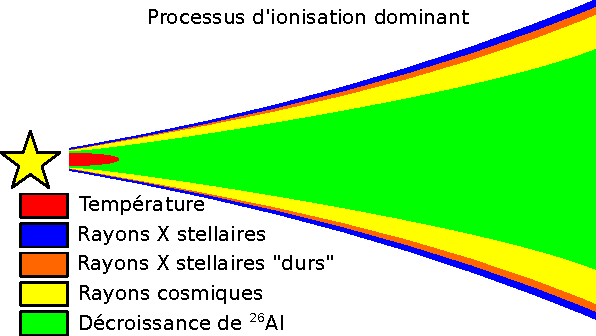
\includegraphics[width=0.49\textwidth]{figure/disk_ionization.pdf}}\hfill
\subfloat[Taux effectif d'ionisation $\zeta_\text{eff}$ par atome d'hydrogène pour un disque avec $\alpha=10^{-2}$ et $\dot{M}=10^{-7}\unit{M_\odot yr^{-1}}$. Les lignes de référence correspondent aux valeurs de $\zeta_\text{eff}$ suivante : $10^{-19}$, $10^{-21}$ et $10^{-23}\unit{s^{-1}}$. Cette figure est basée sur la figure 6 de \cite{ilgner2006ionisation1}.]{\label{fig:ilgner_ionisation}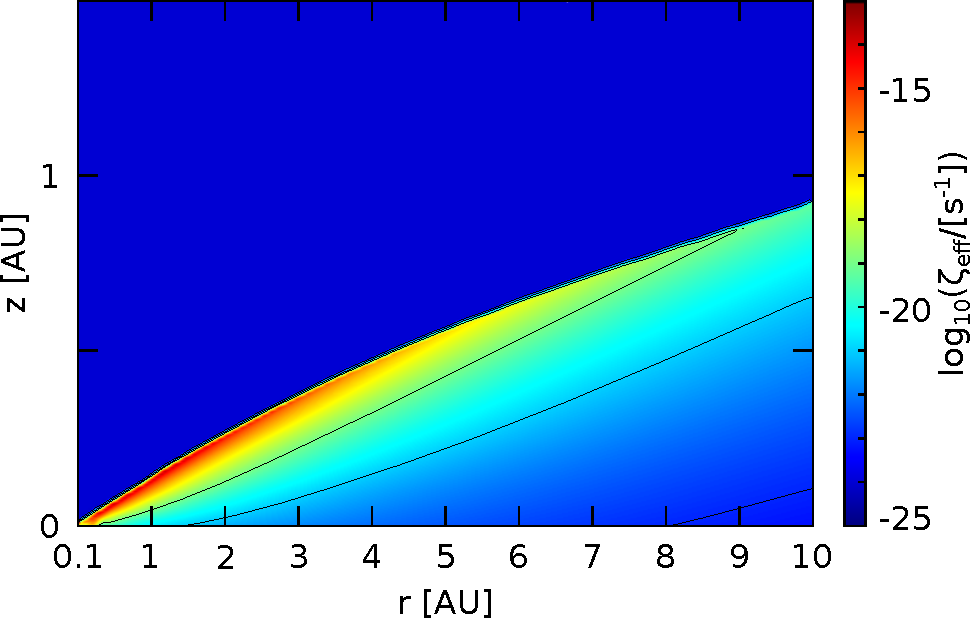
\includegraphics[width=0.49\textwidth]{figure/ilgner_ionization_rate.pdf}}
\caption[Ionisation dans un disque protoplanétaire]{Représentation de l'ionisation dans un disque protoplanétaire}
\end{figure}

On voit donc que les modèles de viscosité constante ou alpha sont incapables de rendre compte de la présence de ces zones de manière intrinsèque. Il est possible de modifier artificiellement les profils de viscosité pour faire apparaître de telles zones mais ça reste \emph{ad hoc}. Dans la suite, je n'ai pas modélisé de zone morte même s'il est probable qu'elles aient un effet sur la migration, le modèle sans zone morte n'est encore pas suffisamment bien compris pour que le rajout de ces zones sans ionisations soit pertinent.

\subsection{La poussière}\index{poussière}
Le disque protoplanétaire est principalement composé de gaz, hydrogène et hélium en majorité. Pourtant, même si la poussière ne représente qu'environ 1\% de la masse du disque elle joue un rôle au moins aussi important que le gaz lui-même.

À cause de la pression quasi-inexistante dans le disque en raison des faibles densités, solide et gaz sont les seules phases
existantes, il n'y a pas de liquide dans l'espace. La poussière représente la matière solide du disque, en grains plus ou moins
fin, allant du nanomètre, micromètre, jusqu'à des tailles planétaires en fin de formation. 

Cette poussière est un composé extrêmement complexe à modéliser. Elle contient différents composés solides en fonction de la température (à certaines températures et densité des composés se volatilisent et d'autres non). La ligne des glaces représente la distance à partir de laquelle de la glace d'eau apparait, augmentant de manière drastique la quantité de poussière dans le disque. 

Le disque évoluant au cours du temps, la ligne des glaces évolue elle aussi à mesure que les propriétés du disque, et en
particulier son profil de densité de gaz, changent \citep{dodsonrobinson2009icelines}.

\bigskip

De plus, la poussière est aussi responsable de l'opacité du disque, c'est-à-dire sa capacité à laisser passer ou non la lumière.
À travers l'opacité, la poussière a donc une influence sur la température du disque qui se refroidit et absorbe le rayonnement
stellaire plus ou moins efficacement. 

\subsection{Opacité du disque}\label{sec:opacity}\index{opacité}
Un paramètre crucial des modèles de disques protoplanétaires est l'opacité du disque qui représente l'absorption du rayonnement incident par une cellule de gaz. Cette dernière dépend principalement de la composition chimique de la poussière sauf quand la température devient suffisamment importante pour que la totalité de la poussière se sublime, généralement au delà de $1500\unit{K}$ \citep{pollack1994composition}, l'opacité étant alors régie par les molécules du gaz.

En fonction de la température et de la pression, différentes espèces se condensent ou se subliment, modifiant les propriétés de la poussière (notamment la quantité de poussière disponible) et donc l'opacité.

L'opacité dépend de plus de la longueur d'onde, les raies d'absorptions n'étant pas uniformément réparties sur toute la gamme de longueur d'onde. Ce dernier paramètre est généralement intégré dans des modèles d'opacité. Citons notamment les opacités moyennes de Planck et de Rosseland, principales opacités utilisées dans les disques. Ce sont des quantités moyennées sur tout un spectre, rendant les opacités indépendantes de la longueur d'onde. 

Dans le cas de l'opacité de la moyenne de Rosseland, on fait l'approximation que le disque est optiquement épais, de sorte qu'on puisse négliger le flux total pour se concentrer uniquement sur la dérivée du flux. C'est-à-dire, en d'autres termes, que seul le flux provenant du gaz environnant arrive jusqu'à la zone considérée, le reste étant absorbé. Dû à l'aspect optiquement épais du disque, on perd l'information sur le flux total, ce qui simplifie les calculs. L'opacité moyenne de Rosseland $\moy{\kappa_R}$ est alors définie comme : 
\begin{align}
\inv{\moy{\kappa_R}} &= \inv{\int_0^\infty \pd{B_\nu}{T}\dif \nu} \int_0^\infty \frac{\pd{B_\nu}{T}}{\kappa_\nu}\dif \nu
\end{align}
où $B_\nu$ et $\kappa_\nu$ sont l'intensité et l'opacité spécifique (dépendant de la fréquence).

À l'inverse, les opacités de Planck concernent les disques optiquement minces, où on ne peut plus considérer uniquement la dérivée du flux. La moyenne est alors effectuée sur l'intensité spécifique directement : 
\begin{align}
\inv{\moy{\kappa_P}} &= \inv{\int_0^\infty B_\nu\dif \nu} \int_0^\infty \frac{B_\nu}{\kappa_\nu}\dif \nu
\end{align}
où $\int_0^\infty B_\nu\dif \nu$ représente l'intensité totale, tandis que $B_\nu$ et $\kappa_\nu$ sont l'intensité et l'opacité spécifique (dépendant de la fréquence).

Dans la pratique, on fait bien souvent l'approximation que le disque est optiquement épais, ce qui est généralement vrai dans les parties internes du disque ($0.1-15\unit{UA}$), lieu de formation des planètes. Pour autant, le calcul des opacités est loin d'être trivial et plusieurs modèles proposent des tables d'opacités dont le détail des propriétés est différent. Le choix du modèle a donc des implications importantes sur le modèle de formation planétaire comme je le détaillerai dans la partie \refsec{sec:influence_opacity_table}. 

En formation planétaire, le modèle le plus utilisé est \citep{bell1994FU}. Mais dans mes études, j'ai utilisé en tout et pour
tout 4 modèles différents \citep{bell1994FU, zhu2009nonsteady, chambers2009analytic, hure2000transition}. À noter que
\citep{bell1994FU, zhu2009nonsteady} sont des modèles qui proposent différentes fonctions analytiques pour définir une opacité
par morceaux. \citep{chambers2009analytic} propose un modèle très simple à opacité constante $\kappa=3\unit{cm^2/g}$ tant que la température
est inférieure à $1380\unit{K}$, puis une simple loi de puissance, fonction uniquement de la température au delà. Enfin, le
modèle dans \citep{hure2000transition} ne définit pas de fonctions par morceaux mais utilise simplement une table d'opacité
fonction de la température et de la densité. L'avantage de ce type de méthode est qu'on ne rajoute pas d'incertitudes par des
ajustements en loi de puissance, c'est donc principalement pour ça que j'ai choisi cette table d'opacité pour mon modèle
standard. 

\subsection{Profil de densité de surface}
Un point crucial dans la modélisation physique d'un disque protoplanétaire est son profil de densité de surface $\Sigma$. Ça signifie d'une part qu'on fait l'approximation d'un disque mince, et que toutes les quantités qu'on considère par la suite sont moyennées selon la direction verticale $z$.

Que l'on fasse évoluer la densité de surface ou non, on doit choisir un profil initial. Ce profil est généralement sous forme d'une loi de puissance de la forme : 
\begin{align}
\Sigma(R) &= \Sigma_0 \cdot \left(\frac{R}{R_0}\right)^{-d}
\end{align}

Un profil largement utilisé est celui de la Masse Minimale de la Nébuleuse Solaire\footnote{MMSN : Minimum Mass Solar Nebulae} \citep{weidenschilling1977distribution, hayashi1981structure}. Dans cet article, le profil de densité est calculé à partir de la masse des planètes. La quantité de solide contenu dans les planètes est répartie dans des anneaux en lieu et place des planètes, puis à partir d'un rapport gaz sur poussière, le profil de densité de surface du gaz est calculé, puis approximé par une loi de puissance, ce qui donne : 
\begin{align}
\Sigma(R) &= 1700 \left(\frac{R}{1\unit{UA}}\right)^{-\sfrac{3}{2}} \unit{g/cm^2}
\end{align}
La première chose à considérer c'est qu'il s'agit d'une masse minimale, c'est-à-dire qu'on suppose que toute
la masse de poussière présente dans le disque de gaz se retrouve dans la masse finale des planètes, ce qui est hautement
improbable, que ce soit à cause notamment de l'accrétion sur l'étoile ou de la disparition d'embryons de planètes soit en
tombant dans l'étoile, soit par éjection du système.

Ce profil est malgré tout une base de travail, vu qu'il est extrêmement difficile de déduire ces informations des observations des disques. Malgré tout, les études semblent montrer que l'on s'attend à un profil moins abrupt que $\Sigma\propto r^{-\sfrac{3}{2}}$, plus proche de $\Sigma\propto r^{-1}$ \citep{bell1997structure}.

%TODO rajouter discussion profils à l'équilibre. 
À partir de l'équation \refeq{eq:diffusion_equation}, on peut considérer le cas particulier des disques à l'équilibre, c'est à dire que $\od{\Sigma}{t}=0$. Ces disques sont alors des disques avec un taux d'accrétion constant $\dot{M}=0$. 

Ces disques à l'équilibre ont deux solutions possibles. Soit on a :
\begin{align*}
\sqrt{R} \dpd{}{R}\left(\nu \Sigma R^\sfrac{1}{2}\right) &= 0
\end{align*}
ce qui donne comme condition :
\begin{align}
\nu \Sigma &= \cte
\end{align}
Le taux d'accrétion, défini comme $\dot{M}=3\pi\nu\Sigma$ est alors constant $\dot{M}=\cte$. 

Soit on a :
\begin{align*}
\nu \Sigma R^\sfrac{1}{2} &= \cte
\end{align*}
ce qui donne : 
\begin{align}
\nu\Sigma &\propto \inv{\sqrt{R}}
\end{align}
Ce qui donne un taux d'accrétion $\dot{M}\propto\inv{\sqrt{R}}$. 

Les deux modèles possibles pour la viscosité, viscosité constante $\nu=\cte$ ou viscosité alpha $\alpha=\cte$ donnent donc 4 solutions différentes (deux chacune) pour les disques à l'équilibre. 

Dans le cas d'une viscosité constante, on a donc un disque avec une densité de surface $\Sigma(R)=\cte$ pour un taux d'accrétion constant, ou $\Sigma(R)\propto R^{-\sfrac12}$ pour avoir $\dot{M}\propto\inv{\sqrt{R}}$.

Dans le cas d'une viscosité alpha, on a $\nu\propto R^{\sfrac12}$. Les deux solutions pour avoir un disque à l'équilibre sont donc $\Sigma(R)\propto R^{-\sfrac12}$ et $\Sigma(R)\propto R^{-1}$. 

En conséquence, un profil $\Sigma(R)\propto R^{-\sfrac12}$ donne un disque à l'équilibre pour les deux modèles de viscosité que j'ai étudié. C'est donc le profil de densité de surface que j'ai privilégié tout au long de ma thèse. 

Mais on voit quand même que l'on a une grande liberté sur la densité de surface du disque, à la fois parce qu'on sait à ce jour peu de chose à ce sujet, mais aussi et surtout parce qu'au cours de son évolution, le disque de gaz va voir sa densité de surface varier énormément. En variant le profil, on étudie donc aussi différentes étapes de formation d'un même disque. 

Le profil de densité de surface, que ce soit au travers de $\Sigma_0$ ou de l'indice $d$ de la loi de puissance a une
grande influence sur les autres paramètres du disque, notamment le profil de température via le chauffage visqueux. 

Il est aussi crucial de garder à l'esprit que la loi de puissance n'est qu'un modèle, issu notamment des observations qui
sondent les parties externes des disques, au delà de plusieurs dizaines d'unités astronomiques. Extrapoler ces lois de puissance
jusqu'aux parties les plus internes est une très grande approximation qui a des conséquences importantes pour les planètes, dont
le lieu de formation se situe vraisemblablement dans les parties internes.

\subsection{Limites et approximations dues à la modélisation}
Tout d'abord, le bord interne est une des parties les plus complexes d'un disque protoplanétaire. Ce bord interne correspond à des zones différentes pour le gaz ou pour la poussière. La poussière disparait quand la température du disque dépasse $1500\unit{K}$ environ, température au delà de laquelle la partie réfractaire des grains se sublime. 

Le gaz, quant à lui, ne se propage pas non plus jusqu'à la surface de l'étoile en raison du champ magnétique important autour des jeunes étoiles. Le bord interne est ainsi déterminé par le rayon de corotation de l'étoile, c'est-à-dire la distance à laquelle une particule en rotation képlerienne orbite à la vitesse de rotation de l'étoile. Le champ magnétique de l'étoile tournant à la vitesse de rotation de l'étoile, ce rayon de corotation correspond ainsi au rayon en dessous duquel le gaz est freiné par le champ magnétique et est rapidement accrété le long des lignes de champ. 

\bigskip

En considérant un système \og étoile + disque\fg isolé, il n'y a pas d'arrêt brutal de la distribution de matière au bord externe qui est donc plutôt une limitation numérique nécessaire aux simulations. La réalité est représentée plus fidèlement par une décroissance continue de la matière, difficile à modéliser tant pour le bord externe que pour la distribution azimutale du disque. 

Généralement, on considère donc que la taille verticale du disque est égale à une échelle de hauteur (grandeur caractéristique de la décroissance exponentielle verticale de la densité de matière), tandis que la taille radiale du disque dépend de la physique que l'on considère. Dans mon cas j'ai souvent pris un bord externe à $100\unit{UA}$.

Je vais ici essayer de récapituler les approximations qui ont été faites jusque-là sur la physique des disques, et qui vont se retrouver implicitement dans tout code qui implémente les équations décrites ci-dessus : 
\begin{enumerate}
\item On suppose que les disques évoluent de manière isolée. Les études suggèrent que les étoiles se forment majoritairement dans des amas (clusters) à l'intérieur desquels la plupart des étoiles font partie de systèmes binaires ou multiples \citep{duquennoy1991multiplicity}. Même si cette approximation permet la modélisation de l'évolution du disque, il est probable que des effets de voisinages aient des conséquences dans tout ou partie des systèmes stellaires, en particulier au travers de la photo-évaporation supplémentaire induite par les étoiles du voisinage.
\item On néglige l'auto-gravité du disque ($M_d \lesssim \frac{H}{R}M_\star$) en considérant que la période où ce n'est pas le cas est courte devant le temps de vie du disque, et que ce dernier tend rapidement vers une configuration où l'auto-gravité est négligeable.
\item On considère que le gaz est en rotation képlerienne $\Omega=\sqrt{\frac{GM_\star}{r^3}}$. Pour cela, on néglige la pression du gaz qui a tendance à rendre la rotation légèrement sous-képlerienne.
\item On considère qu'il n'y a pas de variation de la gravité due à la variation de masse de l'étoile induite par l'accrétion. Ça entraîne alors $\pd{\Omega}{t} = 0$.
\item Dans le calcul du chauffage visqueux, on néglige la vitesse azimutale, la vitesse radiale ainsi que toutes les dérivées en
$\varphi$ compte tenu que le disque est axisymétrique.
\item On se place dans le cadre d'un disque optiquement épais quand on choisit d'utiliser des moyennes de Rosseland pour
l'opacité. Si c'est physiquement cohérent avec les parties internes du disque, ça ne l'est parfois plus dans les parties
externes, surtout si le disque est très étendu.
\item Le modèle d'opacité a une grande influence sur la physique du disque. En particulier, chaque modèle fait des hypothèses sur la métallicité, les propriétés de la poussière, notamment la taille des grains. Chacune de ces hypothèses joue sur l'opacité d'une manière qui est totalement masquée dans les équations ou tables qu'on utilise pour rendre compte de la dépendance de l'opacité en fonction de la température et de la densité.
\item On fait souvent l'approximation que la masse moléculaire moyenne $\mu$ est constante (et typiquement égale à $\mu=2.35$). Or en fonction des transitions d'opacité, la quantité de poussière va brusquement varier, engendrant une variation de $\mu$. Cette masse moléculaire moyenne a en particulier une importance dans le calcul de l'échelle de hauteur $H$ du disque et la vitesse du son $c_s$. 
\item Définir le profil de densité de surface du disque comme une loi de puissance reste une approximation. Ça l'est d'autant plus que le disque est étendu. Du reste, la masse du disque et l'indice de la loi de puissance sont peu contraints, donnant une grande liberté dans le profil de densité dont il faut tenir compte pour mettre en perspective les résultats que l'on obtient.
\item Le modèle choisi pour la viscosité, constante ou prescription alpha, néglige bien souvent la présence de zone morte où
l'ionisation n'est pas suffisante pour que l'on puisse définir une viscosité turbulente. L'absence de ces zones dans un disque
modélisé est bien entendue une approximation à des fins de simplification, mais masque certaines propriétés intrinsèques des
disques dont les conséquences sur la formation planétaire sont encore mal connues.
\item Une dernière approximation, et qui a des conséquences importantes pour l'opacité, le profil de température, la viscosité et par extension, toute la physique du disque, est le fait de considérer les propriétés de la poussière comme figées dans le temps. Au cours de la vie du disque, la poussière évolue. Sa distribution de taille change, la quantité totale de poussière est modifiée, notamment par l'accrétion. Et enfin, à mesure que la poussière se retrouve dans des embryons de planète de plus en plus gros, la quantité de poussière disponible sous la forme de petites particules diminue d'autant. 
\end{enumerate}

\section{Interaction disque-planète}
On ne peut étudier séparément le disque ou les planètes, c'est un système global, en interaction, qui évolue depuis la formation du disque (et les poussières qu'il contient) jusqu'à la dissipation du disque (et la possible présence d'une ou plusieurs planètes).

Je vais maintenant présenter les interactions principales entre les planètes et le disque qui les contient. 

\subsection{Migration des planètes de faible masse : Type I}\label{sec:type_I}
\index{migration!Type I}
Ce type de migration ne concerne que les planètes de faible masse (jusqu'à environ $10M_{\oplus}$) pour lesquelles l'interaction de marée entre la planète et le disque a une réponse linéaire, c'est-à-dire que le profil de densité surfacique n'est quasiment pas modifié par la planète. Ces planètes, qui ne creusent pas de sillon (gap) dans le disque de gaz, vont migrer vers l'intérieur. On appelle cette migration la \gras[migration!Type I]{migration de Type I}.

%\begin{remarque}
%Pour plus de détails, se référer au chapitre 9, page 188--191 de \cite{barnes2010formation} ou \cite{ward1997protoplanet} pour l'article original.
%\end{remarque}

\subsubsection{Couple du disque sur la planète}
Un couple gravitationnel représente l'échange de moment cinétique associé à une force gravitationnelle.  Le couplage gravitationnel entre
les ondes de densité et la planète qui les crée aboutit à un couple qui agit sur la planète : 
\begin{align}
\Gamma &= - \iint_\text{disc} \left(\vect{r}\wedge\grad{\Phi_p}\right)\Sigma r \dif r \dif \theta
\end{align}

À chaque fois qu'il sera mentionné \og couple\fg, celui-ci fera référence au couple \emph{du} disque \emph{sur} la planète.

Ainsi, si le couple est négatif (sous-entendu du disque sur la planète), le disque va prendre du moment cinétique à la planète qui va ainsi migrer plus proche de son étoile, vu que son moment cinétique diminue.\index{migration}

Si le couple est positif, la planète migre vers l'extérieur, cette dernière prenant du moment au disque.

\subsubsection{Couple de Lindblad}\index{couple!de Lindblad}
La présence d'une planète dans un disque de gaz entraine la création d'ondes de densité aux \gras[résonance!de
Lindblad]{résonances de Lindblad} \citep{goldreich1979excitation}. Le couplage gravitationnel entre les ondes de densité et la
planète qui les crée aboutit à un \gras{couple} qui agit sur la planète.

\bigskip

Il est tout d'abord intéressant de remarquer l'origine des bras spiraux dans les galaxies. Ce sont essentiellement des phénomènes statistiques que l'on peut résumer en deux points : 
\begin{enumerate}
\item Une onde de densité se forme par la présence de sur-densités locales comme des nuages de gaz géants
\citep{donghia2013self}. Une fois formée, il est possible que l'onde de densité s'auto-entretienne en modifiant les
excentricités des éléments qui la composent \citep{binney2008book}.

\item L'onde ainsi créée n'est pas une onde matérielle rigide en rotation, mais une onde de densité statistique. Le bras spiral n'est ainsi pas constitué d'une population fixe d'étoile. Les étoiles constituant le bras spiral changent avec le temps, mais statistiquement, la position des étoiles dans la galaxie dessine une onde de densité où le nombre d'étoiles est plus grand. 
\end{enumerate}

\reffig{fig:spiral_arms} schématise l'apparition d'onde de densité. Dans le cas à gauche, des orbites concentriques parfaitement
circulaires sont ajoutées. On ne voit rien de particulier. Par contre, dans le cas à droite, on choisit des orbites très
légèrement excentriques. À chaque étape, on rajoute une orbite en agrandissant l'orbite précédente et en la tournant légèrement.
On voit ainsi apparaître deux ondes de densité dans le disque simplement dues à l'orientation des orbites excentriques.

Ça signifie en particulier que la vitesse de rotation de l'onde de densité n'est pas liée à la vitesse de rotation des étoiles qui la composent. Ceci permet de résoudre le \og winding problem\fg c'est-à-dire le fait que si l'onde de densité était rigide, elle s'enroulerait sur elle-même au bout de quelques orbites seulement, ce qui n'est pas le cas ici \citep{binney2008book}.

\begin{figure}[htbp]
\centering
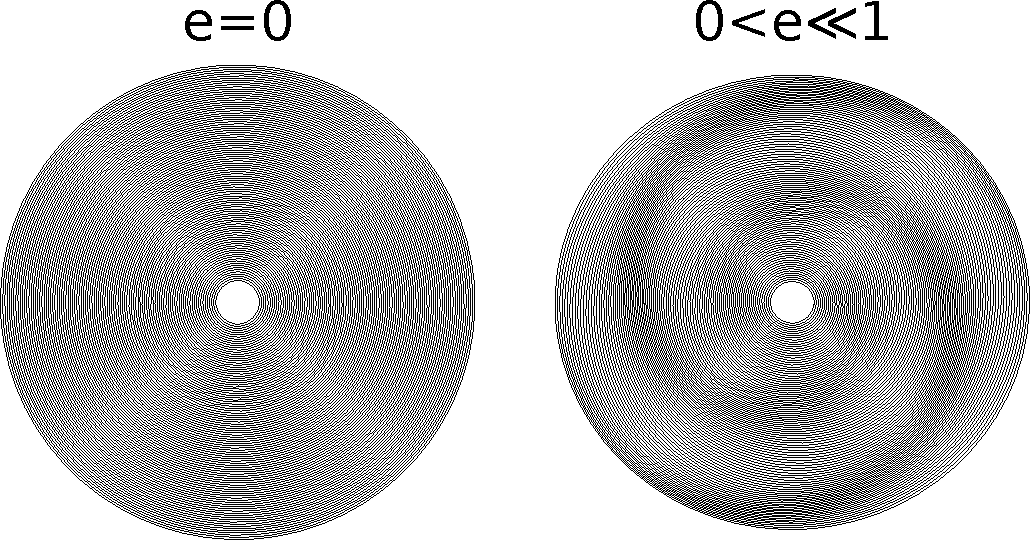
\includegraphics[width=0.9\linewidth]{figure/spiral_arms.pdf}
\caption[Origine des bras spiraux dans une galaxie.]{Illustration de l'origine des bras spiraux dans une galaxie au travers de
l'excitation cohérente de l'excentricité par les bras eux-mêmes. Dans le cas \og $e=0$\fg, les orbites des étoiles, représentées
par les traits noirs sont des cercles parfaits. Dans le cas \og $0<e\ll 1$\fg, les orbites sont toutes très légèrement
excentriques, et les arguments du périhélie légèrement décalés à mesure que les demi-grands axes
augmentent.}\label{fig:spiral_arms}
\end{figure}

\bigskip

Pour l'interaction entre une planète et un disque protoplanétaire, c'est exactement le même principe. Le potentiel de la planète excite les excentricités des éléments fluides voisins jusqu'à former une onde de densité autour de la planète. La différence principale est que le perturbateur est un potentiel gravitationnel tournant, ce qui modifie la forme des ondes de densité comme illustré \reffig{fig:lindblad_torque}. 

\begin{figure}[htbp]
\centering
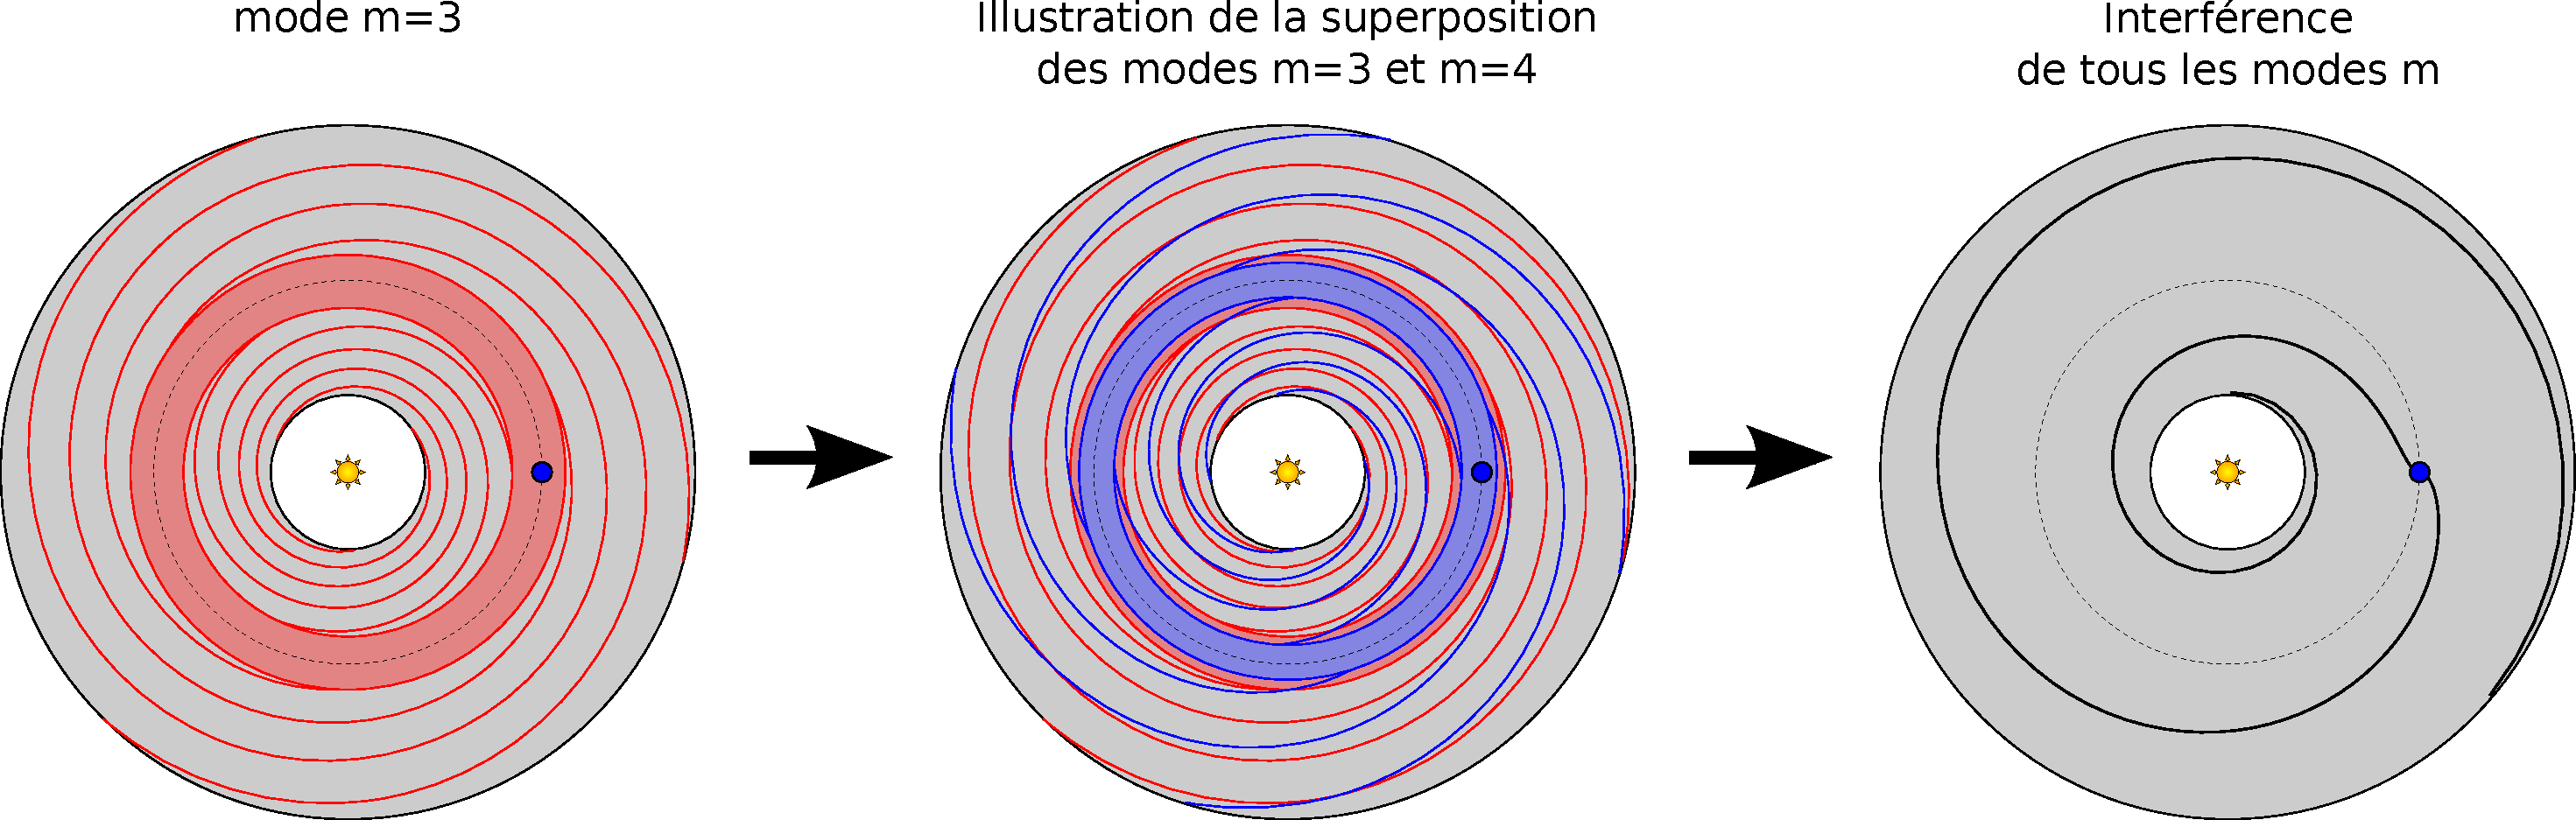
\includegraphics[width=\linewidth]{figure/lindblad_torque.pdf}
\caption[Construction de l'onde de densité due à la présence d'une planète.]{Génération d'ondes de densité dans le disque
protoplanétaire dû à la présence d'une planète. Chaque mode $m$ émet $m$ ondes de densité de part et d'autre de la position
radiale de la planète. Un anneau interne aux positions du mode $m$ est dénué de toute onde dû à ce même mode. Les interférences
entre toutes les ondes de densité de tous les modes donne deux ondes de densité que l'on observe dans des simulations
hydrodynamiques. Les positions successives des interférences constructives sont données par \cite[eq. (13) et
(24)]{ogilvie2002wake}}\label{fig:lindblad_torque}
\end{figure}


% discussion avec laurent : L'explication de l'onde de densité avec les excentricités est correct. Ça permet de résoudre le problème du "winding problem", c'est-à-dire que si le bras spiral était rigide, il serait censé s'enrouler sur lui-même au fil de la rotation (vu que la rotation du bras est égale à la rotation des étoiles qui le composent), et donc au bout de quelques rotations, le bras devrait e^tre hyper enroulé. par contre, si on considère une onde de densité, qui n'existe que statistiquement, ça veut dire que les étoiles entre et sortent du bras, qui lui tourne à une vitesse qui lui est propre, et qui n'a rien à voir avec la vitesse des étoiles en elle même. La majorité des galaxies spirales sont barrées, et on pense que c'est la barre quie st à l'origine des spirales, qui démarrent au bout de la barre.

%Par un phénomène résonnant entre une cellule de gaz et un mode $m$ du potentiel gravitationnel de la planète dont on a décomposé l'expression en série de fourrier (on fait ainsi apparaître des termes de fréquence différen

Le potentiel gravitationnel de la planète peut se décomposer en série de Fourier où chaque mode $m$ (entier) a une dépendance sinusoïdale en azimut et possède $m$ maxima et $m$ minima. 

Pour chaque mode $m$ du potentiel gravitationnel de la planète, on définit deux résonances, une résonance interne (ILR : Inner Lindblad Resonance) et une résonance externe (OLR : Outer Lindblad Resonance) associées aux positions suivantes dans le cas d'un disque froid ($H/R\ll 1$ ; \cite{ward1997protoplanet}) : 
\begin{subequations}
\begin{align}
r_{OLR}(m) &= \left(\frac{m+1}{m}\right)^\sfrac{2}{3}r_p\\
r_{ILR}(m) &= \left(\frac{m-1}{m}\right)^\sfrac{2}{3}r_p
\end{align}
\end{subequations}

Pour un mode $m$ donnée, à partir des anneaux de rayon $r_{ILR}(m)$ et $r_{OLR}(m)$ vont être lancées $m$ ondes de densité. 

Dans le cas des bras spiraux dans une galaxie, c'est principalement un mode $m=2$ qui propage une onde spirale de part et d'autre d'une barre centrale source des ondes de densité. Dans le cas d'une planète dans un disque, des ondes de densité sont lancées pour chaque mode $m$. 

Par interférence constructive \citep{ogilvie2002wake}, la somme de toutes les ondes de densité émises par tous les modes du
potentiel gravitationnel résulte en la formation d'une onde de densité résultante \reffig{fig:lindblad_torque}. 

\bigskip

Il est important de remarquer que la position de la résonance externe d'ordre $m$ est systématiquement plus proche que la résonance interne associée. Ainsi, en sommant sur tous les modes, on arrive à la conclusion que le couple total externe l'emporte toujours sur le couple total interne \citep{ward1997protoplanet}. 

Ainsi, le couple de Lindblad est généralement négatif pour des modèles typiques de disques protoplanétaires \citep{ward1997protoplanet}.

La résolution numérique des équations linéarisées permet de trouver une formule analytique pour le couple de Lindblad $\Gamma_L$. Dû à la résolution numérique qui doit s'affranchir de la divergence du potentiel gravitationnel en $r=r_0$, cette formule introduit une longueur de lissage permettant de contourner la singularité du noyau du Green du potentiel gravitationnel \citep[eq. (14)]{paardekooper2010torque} : 
\begin{align}
\gamma \Gamma_L/\Gamma_0 &= - \left(2.5 +1.7\beta -0.1d\right) \left(\frac{0.4}{b/h}\right)^{0.71}\label{eq:lindblad-torque}
\end{align}
où $\gamma$ est l'indice adiabatique, $b/h$ le paramètre de lissage du potentiel gravitationnel, et $\beta$ et $d$ sont les négatifs des exposants des lois de puissance pour les profils de température ($T \propto R^{-\beta}$) et de densité de surface ($\Sigma \propto R^{-d}$). 

Le couple est ici exprimé en unité de $\Gamma_0$, couple de référence défini par : 
\begin{align}
\Gamma_0 &= \left(\frac{q}{h}\right)^2\Sigma_p {r_p}^4 {\Omega_p}^2
\end{align}

Notons aussi que le processus physique du transport du moment cinétique de la planète est réalisé par l'onde de densité. Le
moment cinétique est emporté par l'onde de densité qui l'échange avec le gaz environnant à mesure que ce dernier amortit et
dissipe l'onde \citep{crida2006width}.

\subsubsection{Couple co-orbital ou de corotation}\index{couple!de corotation}\label{sec:couple-corotation}
\begin{figure}[htbp]
\centering
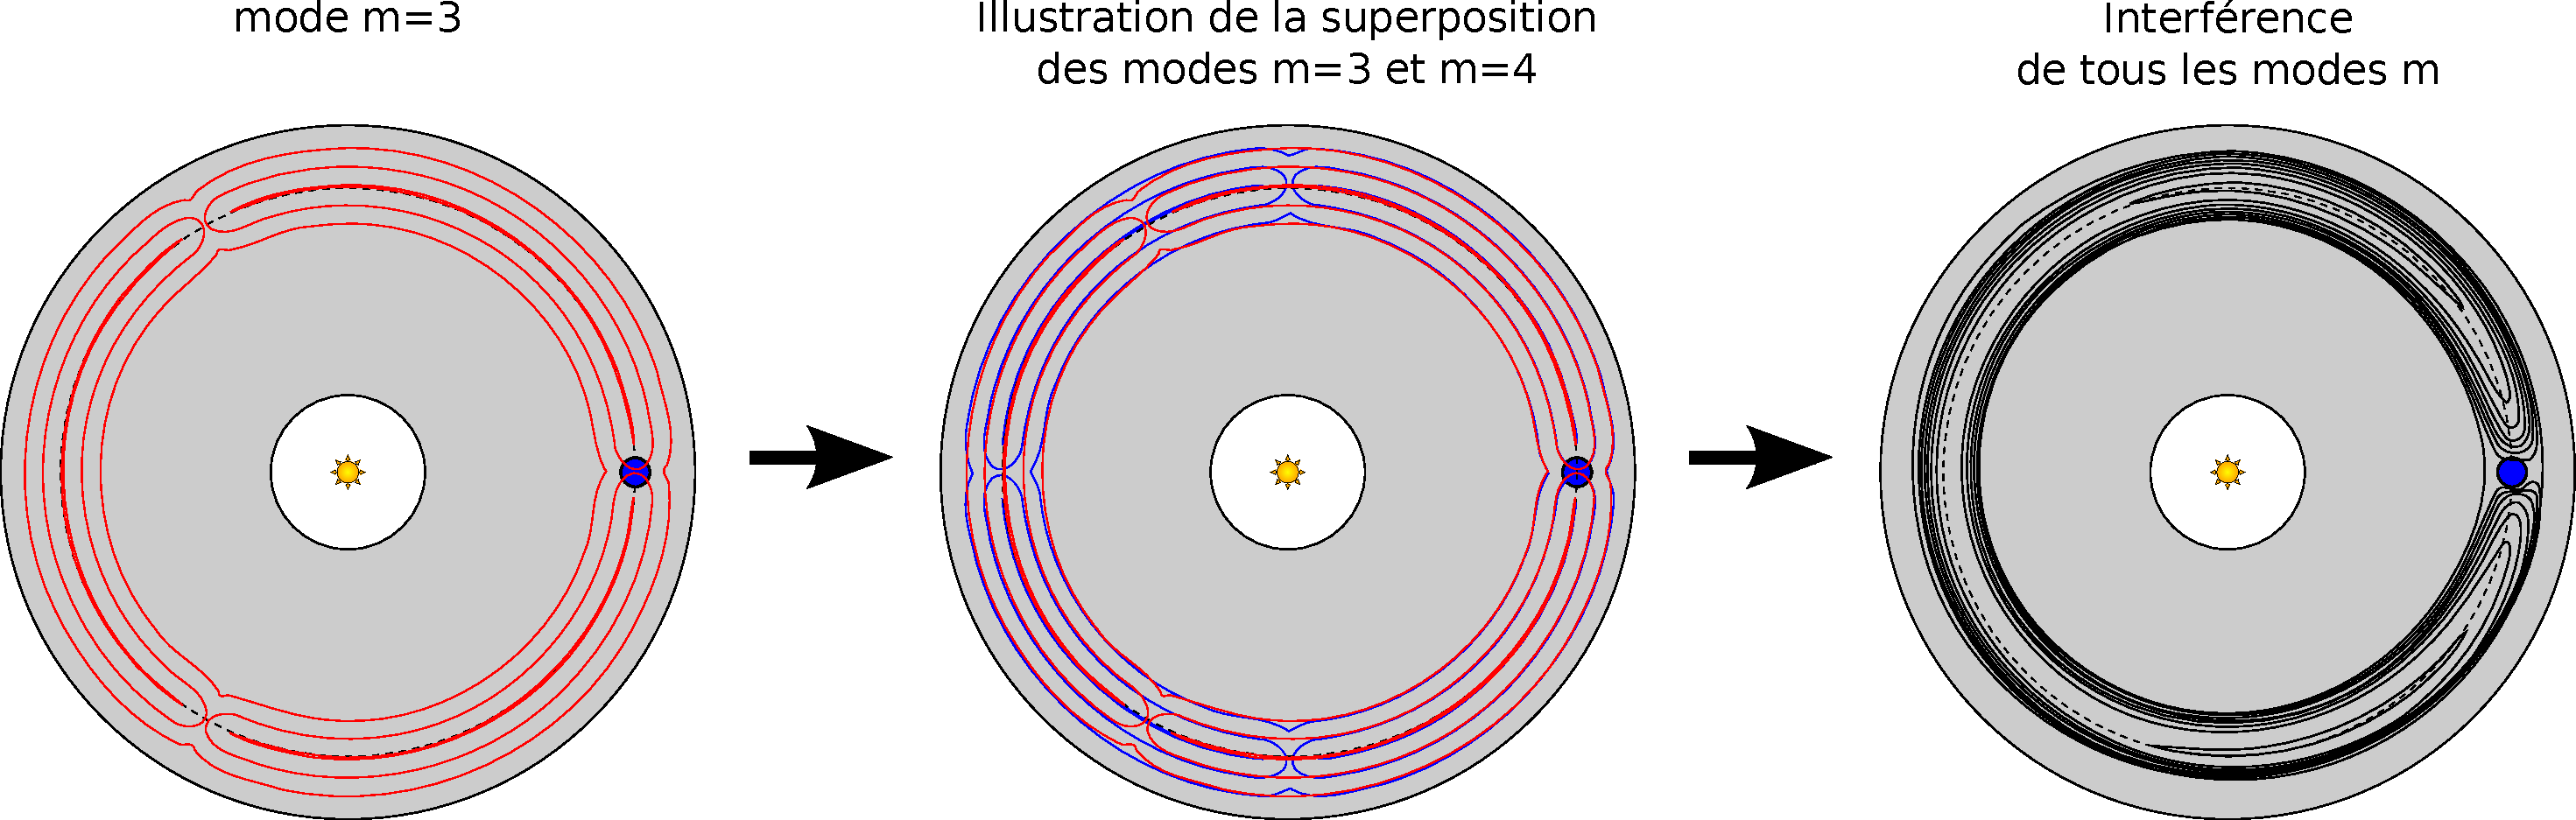
\includegraphics[width=\linewidth]{figure/corotation_modes.pdf}
\caption[Zone de corotation d'une planète.]{À partir de la décomposition en série de Fourier du potentiel
gravitationnel de la planète, chaque mode $m$ a pour conséquence $m$ zones de libration dans la zone de corotation avec la
planète. Les interférences entre l'infinité de modes $m$ fait apparaître des orbites fer-à-cheval (\og horseshoe orbits\fg) dans
le référentiel tournant avec la planète. La zone de corotation a ici été exagérée pour plus de
lisibilité.}\label{fig:corotation_torque}
\end{figure}

De la même manière que précédemment pour le couple de Lindblad, on peut repartir de la décomposition en série de Fourier du potentiel gravitationnel de la planète. Pour chaque mode $m$ de la décomposition, on voit apparaître $m$ zones de libration, centrées sur le rayon de la planète, et réparties en azimut. \reffig*{fig:corotation_torque} représente le mode $m=3$, puis une juxtaposition de mode et finalement le résultat des interférences constructives entre tous les modes $m$ de la décomposition.


Le couple de corotation provient des échanges gravitationnels que va avoir une particule fluide en co-orbite avec une planète. Il existe deux types de couples, issus du gradient de deux quantités physiques distinctes, la vorticité spécifique (vorticité divisée par la densité de surface) appelée parfois vortensité et l'entropie. 

Chacun de ces deux couples possède une partie qui peut saturer en fonction des conditions physiques. 

Pour illustrer le principe de la saturation, et sans considérer un couple en particulier, il convient de définir certains temps caractéristiques afin de comprendre l'origine de ce couple non saturé, et pourquoi ce dernier peut saturer. \reffig*{fig:corotation_orbits} représente schématiquement les 3 temps principaux mis en jeux. 

\begin{figure}[htbp]
\centering
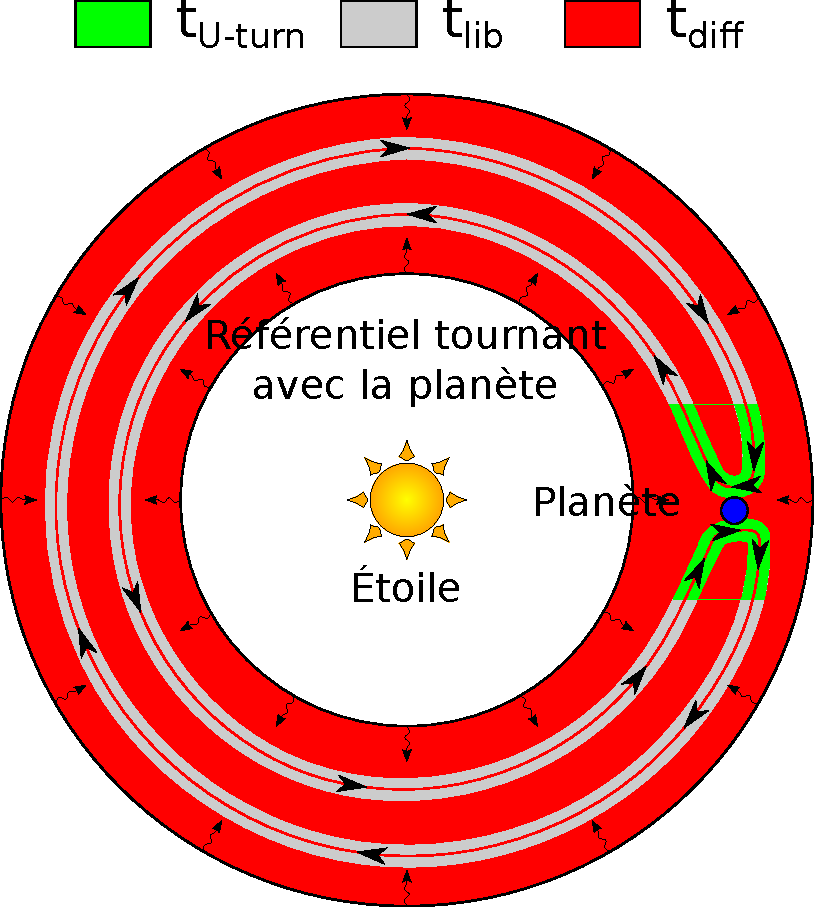
\includegraphics[width=0.75\linewidth]{figure/corotation_times.pdf}
\caption[Temps caractéristiques mis en jeu dans la zone de corotation.]{Dans le référentiel tournant avec la planète (qui est
donc fixe dans ce repère), représentation d'une orbite de corotation ainsi que des différents temps caractéristiques mis en
jeux. $t_\text{lib}$ est le temps mis par un élément fluide pour effectuer une orbite de corotation. $t_\text{U-turn}$ est le
temps mis par un élément fluide pour effectuer un demi-tour devant la planète. $t_\text{diff}$ peut être suivant le cas le temps
radiatif $t_\text{rad}$ ou le temps visqueux $t_\text{vis}$ nécessaire pour homogénéiser les propriétés thermodynamiques de
l'élément fluide avec son environnement.}\label{fig:corotation_orbits}
\end{figure}

On définit tout d'abord $t_\text{lib}$ comme le temps mis par un élément fluide pour effectuer une co-orbite complète dans la zone de fer-à-cheval. Ceci dépend de la distance de l'élément fluide au rayon de corotation. Mais le temps de libration le plus court est obtenu à la distance $x_s$ de la corotation, et vaut \citep[eq. (52)]{baruteau2008corotation} : 
\begin{align}
t_\text{lib} &= \frac{4\pi}{x_s\abs{\od{\Omega}{r}}} = \frac{8\pi r_p}{3\Omega_p x_s}
\end{align}
où $x_s$ est la demi-largeur de la zone de fer-à-cheval (\og half-width of the horseshoe region\fg) \citep[eq. (44)]{paardekooper2010torque} :
\begin{align}
\frac{x_s}{r_p} &= \frac{1.1}{\gamma^{1/4}} \left(\frac{0.4}{b/h}\right)^{1/4} \sqrt{\frac{q}{h}}
\end{align}
Dans le cas d'une planète de $20\unit{M_\oplus}$ à $1\unit{UA}$ dans un disque avec $h=0.05$ et $M_\star=1M_\odot$, ce temps de libration vaut $t_\text{lib}\sim 38 p_\text{orbital}$. 

Le temps $t_\text{U-turn}$ représente quant à lui la durée nécessaire à un élément fluide pour effectuer un demi-tour devant la
planète, c'est-à-dire pour parcourir la zone de longueur $2x_s$\footnote{$x_s$ est la demi-largeur de la zone de fer-à-cheval
(\og half-width of the horseshoe region\fg)} devant la planète. Il est défini par \citep[eq. (64)]{baruteau2008corotation}
\begin{align}
t_\text{U-turn} &\simeq \frac{4}{\Omega_p}\left[\frac{H(r_p)}{R_H}\right]^\sfrac{3}{2}
\end{align}
où $R_H=r_p (q/3)^{1/3}$ est le rayon de Hill de la planète. Dans le cas d'une planète de $20\unit{M_\oplus}$ à $1\unit{UA}$ dans un disque avec $h=0.05$ et $M_\star=1M_\odot$, ce temps vaut $t_\text{U-turn} \sim 1.6 p_\text{orbital}$.

Un troisième et dernier temps $t_\text{diff}$ rentre en jeu, c'est le temps de diffusion. Selon le processus physique mis en
jeu, ce temps peut être $t_\text{rad}$ ou $t_\text{visc}$.

$t_\text{rad}$ représente le temps de diffusion par refroidissement radiatif. Ce temps est plus long quand on se rapproche de l'étoile car le rayonnement est plus rapidement réabsorbé. Le temps radiatif au travers de la zone de corotation est de l'ordre de :
\begin{align}
t_\text{rad} &= \frac{{x_s}^2}{\chi}
\end{align}
où $x_s$ est la demi-largeur de la zone de corotation et $\chi$ est la diffusivité thermique.
 
$t_\text{visc}$ représente la diffusion d'une quantité physique par la viscosité. Ce temps est plus court quand on se rapproche de l'étoile. Le temps visqueux à la zone de corotation $t_\text{visc}$ est  de l'ordre de \citep{masset2001coorbital, masset2002coorbital, ogilvie2003saturation}
\begin{align}
t_\text{visc} &\sim \frac{{x_s}^2}{\nu}
\end{align}

Quand la grandeur physique considérée est la vortensité (ou vorticité spécifique), seul $t_\text{visc}$ est à prendre en compte. Quand c'est l'entropie, les deux temps $t_\text{visc}$ et $t_\text{rad}$ sont importants. \reffig*{fig:corotation_orbits} récapitule les temps mis en jeux et à quoi ils correspondent.

\bigskip

Pour que le couple de corotation soit non saturé, on doit satisfaire aux inéquations suivantes \citep[eq. (31)]{baruteau2013recent} :
\begin{align}
t_\text{U-turn} < t_\text{diff} < \frac{t_\text{lib}}{2}
\end{align}
$t_\text{U-turn}$ est le temps nécessaire pour faire le demi-tour devant la planète (pour traverser une zone égale approximativement à $2x_s$). $t_\text{lib}$ est le temps de libration, c'est-à-dire le temps mis par une particule fluide pour faire le tour de la zone en fer-à-cheval. $t_\text{diff}$ quant à lui est le temps de diffusion de la quantité physique considérée. Suivant les cas, il peut y avoir plusieurs temps de diffusion qui sont importants, auquel cas les inégalités doivent être satisfaites pour tous les temps de diffusions mis en jeux.

\begin{figure}[htbp]
\centering
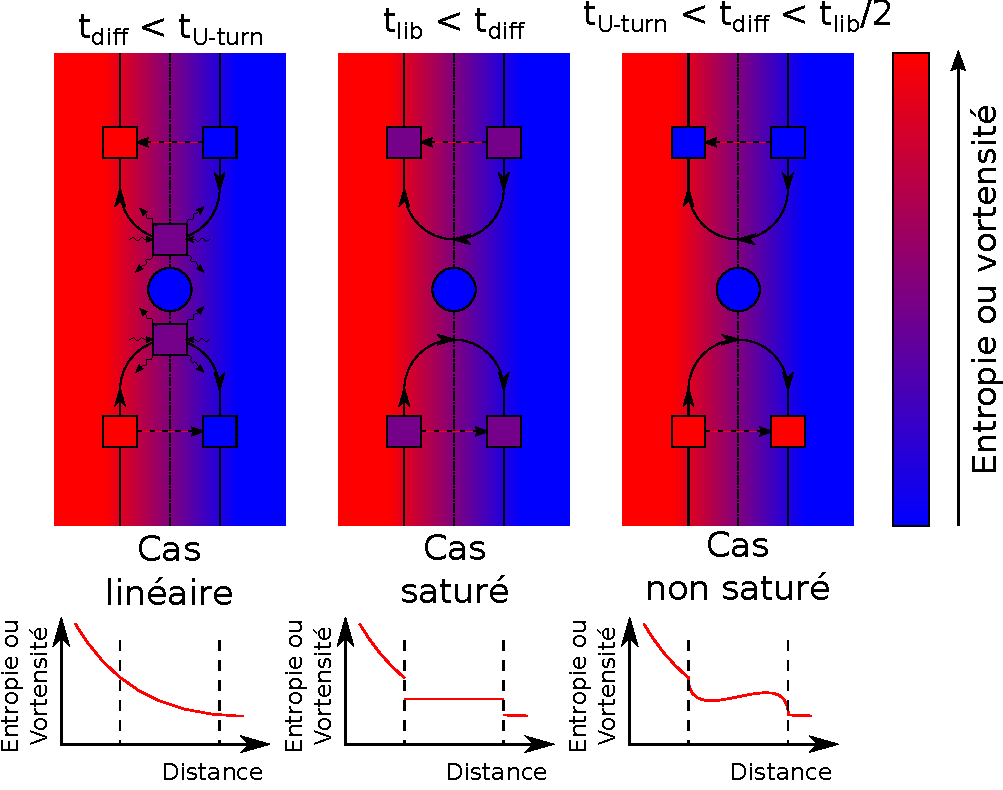
\includegraphics[width=0.75\linewidth]{figure/corotation_principle.pdf}
\caption[État du couple de corotation en fonction des valeurs des temps caractéristiques.]{Dans le référentiel tournant avec la
planète, représentation du mécanisme général à l'origine du couple de corotation. Lorsque les temps de diffusion $t_\text{diff}$
sont plus grands que le temps de libration $t_\text{lib}$, le couple de corotation sature car le gradient de vortensité/entropie
au travers de la région fer-à-cheval tend à s'aplatir. Ce dernier est restauré quand les temps de diffusion $t_\text{diff}$ sont
plus courts que le temps de libration $t_\text{lib}$. Dans ce cas, la valeur optimale du couple de corotation est obtenue
lorsque les temps de diffusion $t_\text{diff}$ sont de l'ordre de la moitié du temps de libration $t_\text{lib}/2$. Dans la
limite où les temps de diffusion $t_\text{diff}$ sont plus courts que le temps de demi-tour $t_\text{U-turn}$, l'amplitude du
couple de corotation décroit pour atteindre la valeur prédite par une analyse linéaire.}\label{fig:corotation_principle}
\end{figure}

\reffig*{fig:corotation_principle} illustre les trois cas possibles en fonction des commensurabilités entre les différents temps caractéristiques mis en jeux.

L'idée générale afin d'éviter la saturation, c'est qu'on doit restaurer le gradient d'entropie / de vortensité au travers de la
zone fer-à-cheval. Il faut donc que les processus diffusifs soient suffisamment efficaces pour qu'en arrivant à la région de \og
U-turn\fg de l'autre côté, l'élément fluide ait pu équilibrer ses conditions physiques avec le milieu environnant. Cette
condition est illustrée par l'inégalité suivante : 
\begin{align}
t_\text{diff} < \frac{t_\text{lib}}{2}
\end{align}

Mais il faut de plus que la diffusion ne soit pas trop efficace, sous peine que la valeur du couple de corotation diminue pour atteindre la valeur prédite par une analyse linéaire. Ceci donne alors la deuxième inéquation : 
\begin{align}
t_\text{U-turn} < t_\text{diff}
\end{align}

\bigskip

De la même manière que pour le couple de Lindblad, la résolution numérique des équations nous permet d'avoir des expressions analytiques pour les couples de corotation. 

Il y a d'une part les couples soumis à saturation \citep[eq. (45)]{paardekooper2010torque} :
\begin{subequations}
\begin{align}
\gamma \Gamma_\text{c,hs,baro}/\Gamma_0 &= 1.1\left( \frac{3}{2} - d\right)\left(\frac{0.4}{b/h}\right)\\
\gamma \Gamma_\text{c,hs,ent}/\Gamma_0 &= \frac{\xi}{\gamma}\left(10.1\sqrt{\frac{0.4}{b/h}} - 2.2\right)\left(\frac{0.4}{b/h}\right)
\end{align}\label{eq:saturated-corotation-torque}
\end{subequations}
et les couples non soumis à saturation, dits linéaires \citep[eq. (17)]{paardekooper2010torque} :
\begin{subequations}
\begin{align}
\gamma \Gamma_\text{c,lin,baro}/\Gamma_0 &= 0.7\left( \frac{3}{2} - d\right)\left(\frac{0.4}{b/h}\right)^{1.26}\\
\gamma \Gamma_\text{c,lin,ent}/\Gamma_0 &= \xi\left[2.2\left(\frac{0.4}{b/h}\right)^{0.71} - \frac{1.4}{\gamma}\left(\frac{0.4}{b/h}\right)^{1.26}\right]
\end{align}\label{eq:linear-corotation-torque}
\end{subequations}
$d$ et $\xi=\beta - (\gamma-1)d$ sont respectivement les négatifs des exposants des lois de puissance pour les profils 1D de densité de surface ($\Sigma\propto R^{-d}$) et d'entropie ($S \propto R^{-\xi}$).

\bigskip

Dans la pratique, ce couple peut être positif (migration vers l'extérieur) ou négatif (migration vers l'intérieur) en fonction
des variations des quantités physiques par rapport à leur valeur nominale.

\subsubsection{Modélisation dans le code N-corps}
Les couples de Lindblad et de Corotation ont été intégrés aux simulations numériques en utilisant le modèle de \cite{paardekooper2011torque}. Plus de détails sur l'implémentation de ces formules et le modèle de disque utilisé dans la section \refsec{sec:code_n-corps}.

\subsection{Migration des planètes massives : Type II}\index{migration!Type II}
Par massive, on entend une planète qui va induire des modifications importantes du profil de densité du disque. L'approximation du régime linéaire n'est alors plus valable. 

Je présente ici très succinctement ce type de migration que je n'ai pas considéré tout au long de ma thèse. Je me place dans le régime linéaire et me suis concentré sur les cœurs de planète géante et les planètes telluriques. J'ai donc négligé tous les effets non-linéaires dû aux grandes masses, et en particulier la création d'un sillon par les planètes.

\bigskip

Quand une planète dans un disque devient suffisamment massive, la réponse du disque n'est plus linéaire, et des ondes de densité induites par la planète forment des chocs non loin de là où elles sont émises. La répulsion entre le disque et la planète devient si forte qu'une cavité annulaire se forme autour de l'orbite de la planète, creusant le disque de gaz \citep{lin1986tidal}.

Une fois que la cavité est formée, la planète est dite en migration de \gras[migration!Type II]{Type II} : son orbite agit alors essentiellement comme une barrière entre les deux parties du disque de gaz, \emph{interne} et \emph{externe}. Du gaz peut sauter le gap \citep{lubow2006gas}, ou être accrété par la planète mais cette dernière voit son mouvement régit par le disque de gaz, se retrouvant entraînée par la migration de celui-ci.

Quand la planète creuse un sillon et que sa masse est inférieure ou de l'ordre de la masse locale du disque ($M_p \lesssim M_\text{d,loc}$ avec lequel elle interagit, alors le temps de migration de la planète est contrôlé par le temps visqueux du disque, car cette dernière se comporte comme une particule de ce disque \citep{nelson2000migration}.

\bigskip

Pendant que le gap dû à la planète est en train de se creuser, un mode de migration intermédiaire apparaît, appelé migration de 
\gras[migration!Type III]{Type III}. Dans certaines conditions, ce mode peut entrainer une migration rapide vers l'intérieur 
\citep{masset2003runaway}. 

\subsection{L'amortissement de l'excentricité et de l'inclinaison}\index{amortissement!excentricité}\index{amortissement!inclinaison}%circularisation
%Penser aux papiers cresswell et al. 2007 et tanaka et al. 2004
Une planète sur une orbite non-circulaire $e\neq 0$ génère des ondes supplémentaires à cause de son excentricité. De même, une orbite légèrement inclinée induit des ondes à cause de l'inclinaison $I$ de la planète. 

Des calculs analytiques sur les équations linéarisées (valables quand $e$ et $I$ sont faibles $e,I \ll H/R$) montrent que les ondes dues à l'excentricité ou l'inclinaison ont tendance à amortir l'élément orbital qui est à leur origine. \cite[eqs. (45), (47)]{tanaka2004three} trouvent un amortissement exponentiel dont les temps caractéristiques sont : 
\begin{subequations}
\begin{align}
\frac{\overline{\dot{e}}}{e} &= -\frac{0.780}{t_\text{wave}}\\
\frac{\overline{\dot{I}}}{I} &= -\frac{0.544}{t_\text{wave}}
\end{align}
\end{subequations}
où le temps caractéristique de l'évolution orbitale $t_\text{wave}$ est donné par \cite[eq. (49)]{tanaka2004three} :
\begin{align}
t_\text{wave} &= \frac{M_\star}{M_p}\frac{M_\star}{\Sigma_p a^2} \left(\frac{H}{R}\right)^4 {\Omega_p}^{-1}
\end{align}

D'une manière générale, le temps caractéristique d'amortissement pour l'excentricité et l'inclinaison est similaire et de l'ordre de \citep{tanaka2004three} :
\begin{align}
\tau_e \sim \tau_I &\sim h^2 t_\text{mig}
\end{align}
où $t_\text{mig}$ est le temps caractéristique de l'évolution orbitale.

Des simulations hydrodynamiques montrent que le même phénomène d'amortissement se produit pour des valeurs plus grandes de $e$ et $I$, tout en étant dans un régime différent que celui à faibles valeurs ($e,I \ll H/R$) \citep{cresswell2007evolution}. On explique cela pour l'inclinaison par le fait qu'à grande inclinaison, la planète peut sortir du disque est ressentir un amortissement réduit. Pour l'excentricité quant à elle, on invoque le fait que durant son orbite la planète va voir sa vitesse varier par rapport à celle du disque de gaz \citep{papaloizou2000orbital}.

\subsection{L'accrétion du gaz}\label{sec:accretion_coeur}\index{accrétion de gaz}
Dans le modèle d'accrétion de cœur, les planètes géantes sont d'abord des cœurs rocheux (ou noyaux) qui grossissent jusqu'à 
atteindre une masse critique de l'ordre de $10 M_{\oplus}$ \citep{pollack1996formation}. Une fois cette masse atteinte, le cœur 
commence à accréter rapidement du gaz jusqu'à former une géante gazeuse.

Ceci implique que la formation des planètes géantes doive se passer avant que le disque de gaz ne se dissipe (ce qui intervient au bout de quelques millions d'années).

La ligne des glaces est une limite radiale virtuelle au delà de laquelle on peut trouver de l'eau sous forme solide ; autour de 
$4\unit{UA}$ \citep{martin2013evolution}. Parce que la quantité de matière disponible pour former les noyaux de planètes géantes 
est plus importante au delà de cette ligne, on pense souvent que la zone au delà est le lieu de la formation des géantes 
gazeuses \citep{sasselov2000snowline}. Pourtant, à l'heure actuelle, il n'est pas certain que cette zone au delà de la ligne 
des glaces soit le lieu de formation des noyaux de planètes géantes. On ne sait pas 
vraiment s'il y a une zone privilégiée ou non, la limite virtuelle de la ligne des glaces pourrait ne pas être valable, la glace 
ne rajoutant qu'environ 50\% de masse en plus \citep{lodders2003solar}.\index{ligne des glaces}


\bigskip

L'accrétion de gaz va peu à peu changer le régime de migration d'une planète. Par migration de \gras[migration!Type I]{Type 
I}, la vitesse de migration est proportionnelle à la masse. Quand la planète devient suffisamment massive pour creuser un 
sillon et migrer par migration de \gras[migration!Type II]{Type II}, la vitesse de migration est gouvernée par la dérive 
radiale du disque de gaz. Enfin, quand la masse de la planète devient comparable à celle du disque, l'inertie de la planète 
commence à jouer un rôle dans sa migration et retarder les variations de migration, normalement gouvernée par l'évolution du 
disque de gaz \citep{crida2007cavity}.

\subsection{Récapitulatif des interactions dans le code N-corps}
Numériquement, le couple de la migration de Type I est pris en compte en utilisant les formules semi-analytiques développées par \cite{paardekooper2011torque}. 

L'amortissement de l'inclinaison et de l'excentricité quant à elles sont modélisées via les formules de 
\cite{cresswell2008three}.

L'accrétion de gaz et la migration de Type II et III n'ont pas été implémentés ici. Nous nous limitons au cas où la masse des 
planètes n'est pas suffisante pour modifier la structure du disque de gaz (réponse linéaire). 
